\documentclass[a4paper]{jsarticle}
\setlength{\topmargin}{-20.4cm}
\setlength{\oddsidemargin}{-10.4mm}
\setlength{\evensidemargin}{-10.4mm}
\setlength{\textwidth}{18cm}
\setlength{\textheight}{26cm}

\usepackage[top=15truemm,bottom=25truemm,left=20truemm,right=20truemm]{geometry}
\usepackage[latin1]{inputenc}
\usepackage{amsmath}
\usepackage{amsfonts}
\usepackage{amssymb}
\usepackage[dvipdfmx]{graphicx}
\usepackage[dvipdfmx]{color}
\usepackage{listings}
\usepackage{listings,jvlisting}
\usepackage{geometry}
\usepackage{framed}
\usepackage{color}
\usepackage[dvipdfmx]{hyperref}
\usepackage{ascmac}
\usepackage{enumerate}
\usepackage{tabularx}
\usepackage{cancel}
\usepackage{scalefnt}

\renewcommand{\figurename}{fig.}
\renewcommand{\tablename}{table }
\newcommand{\redunderline}[1]{\textcolor{BrickRed}{\underline{\textcolor{black}{#1}}}} 

\hypersetup{
	colorlinks=false, % リンクに色をつけない設定
	bookmarks=true, % 以下ブックマークに関する設定
	bookmarksnumbered=true,
	pdfborder={0 0 0},
	bookmarkstype=toc
}

\lstset{
basicstyle={\ttfamily},
identifierstyle={\small},
commentstyle={\smallitshape},
keywordstyle={\small\bfseries},
ndkeywordstyle={\small},
stringstyle={\small\ttfamily},
frame={tb},
breaklines=true,
columns=[l]{fullflexible},
xrightmargin=0zw,
xleftmargin=3zw,
numberstyle={\scriptsize},
stepnumber=1,
numbersep=1zw,
lineskip=-0.5ex
}



\author{}
\title{大学院入試対策}
\date{}

\begin{document}
\maketitle

\section{基本知識}
\subsection{平方根}
\begin{itembox}[l]{Point}
    \begin{center}
        平方根をはずすときは,\textgt{絶対値}がつく
    \end{center}
\end{itembox}
\begin{eqnarray*}
    \sqrt{a^2}=|a|
\end{eqnarray*}
\subsection{対数の変換公式}
\begin{itembox}[l]{変換公式}
    \begin{eqnarray*}
        \log_ab=\frac{\ln b}{\ln a}\\
    \end{eqnarray*}
\end{itembox}
\subsection{重心}
\begin{itembox}[l]{重心}
    \begin{eqnarray*}
        x_G=\dfrac{\Sigma\; mx}{\Sigma\; m}=\dfrac{微小領域に作用するモーメントの総量}{総質量}\\
    \end{eqnarray*}
\end{itembox}
\subsection{動滑車}
\begin{figure}[htbp]
    \begin{center}
        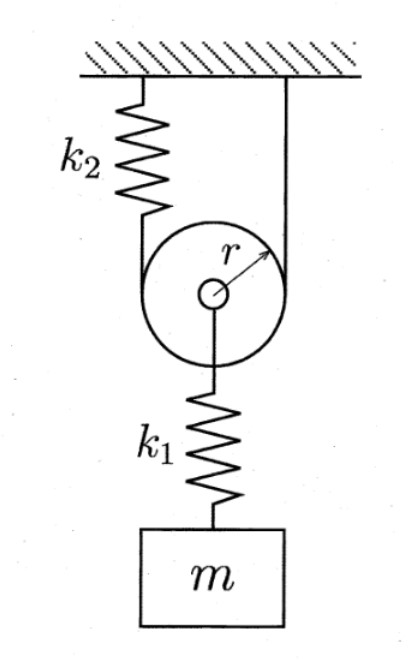
\includegraphics[width=50mm]{images/kiriki_image1.jpg}
        \caption{H20 試験問題 [3]}
    \end{center}
\end{figure}
\begin{itembox}[l]{動滑車}
    \begin{center}
        持ち上げるのに必要な力は$1/2$倍,その移動距離は$2$倍
    \end{center}
\end{itembox}
\subsection{正規化}
データを一定の規則に基づいて変形し,利用しやすくすること.
\subsection{逆三角関数}
\begin{itembox}[l]{$\mathrm{Tan}^{-1}$ (アークタンジェント)}
    \begin{center}
        $\tan$の逆関数のこと\\
        範囲は$-\dfrac{\pi}{2}\leq x \leq\dfrac{\pi}{2}$
    \end{center}
\end{itembox}
\subsection{単位ベクトル}
\begin{itembox}[l]{単位ベクトル}
    \begin{center}
        長さ $1$ のベクトルのこと
    \end{center}
\end{itembox}
\newpage
\section{線形代数}
\subsection{行列}
\subsubsection{行列演算の性質}
基本的には,普通の計算と同じ.
ただし,\textgt{積}には注意が必要.
\begin{itembox}[l]{行列演算特有の性質}
    \begin{eqnarray*}
        \left(AB\right)C&=&A\left(BC\right)\\
        A\left(B+C\right)&=&AB+AC\\
        \left(A+B\right)&=&AC+BC\\
        AB&\neq& BA
    \end{eqnarray*}
    ※ 積をとる順番に注意する\\
    ※ 積の交換法則のみ成り立たない
\end{itembox}
\subsection{一次独立・一次従属}
\begin{itembox}[l]{一次独立}
    \begin{center}
        $c_1a_1+c_2a_2+\cdots+c_ka_k=0$ を満たすのが $c_1=c_2=\cdots=c_k=0$の場合に限るとき,
        \textgt{一次独立である}という.
    \end{center}
\end{itembox}
\begin{itembox}[l]{一次従属}
    \begin{center}
        $c_1a_1+c_2a_2+\cdots+c_ka_k=0$ を満たすのが $c_1=c_2=\cdots=c_k=0$の場合でないとき,
        \textgt{一次従属である}という.
    \end{center}
\end{itembox}
\begin{itembox}[l]{物理的な意味}
    ある2つのベクトル$a,b\left(a\neq 0,b\neq 0\right)$が存在し,
    それらが並行でない$\left(a\not\parallel b\right)$とき,\textgt{一次独立である}という.\\
    また,それらが,平行である$\left(a\parallel b\right)$とき,\textgt{一次従属である}という.
\end{itembox}
\begin{itembox}[l]{一次独立の判定}
    ベクトルの線形独立・線形従属の判定は,$c_1a_1+c_2a_2+\cdots+c_ka_k=0$を満たす
    $c_1,c_2,\cdots,c_k$の値を調べることで行われる.すなわち, $c_1,c_2,\cdots,c_k$に対する
    \textgt{連立一次方程式を解くこと}に帰着される
\end{itembox}
\subsection{連立一次方程式}
\begin{itembox}[l]{行列の基本変形}
    \begin{enumerate}[(1)]
        \item 1つの行を何倍か($\neq0$倍)する
        \item 2つの行を入れ替える
        \item 1つの行にほかの行の何倍かを加える
    \end{enumerate}
\end{itembox}
\begin{itembox}[l]{消去法による解法}
    \begin{enumerate}[(1)]
        \item 連立一次方程式より拡大係数行列を抽出(行列のデータ化)
        \item 抽出した拡大係数行列を簡約化する(未知数の整理)
        \item 簡約化の結果を連立一次方程式に還元し解を作成する
    \end{enumerate}
\end{itembox}
\begin{itembox}[l]{解が不定の場合}
    「1式に1未知数」という形は,一般には成り立たない.そこで,「1式に1未知数」に近い形に整理したものが\textgt{階段行列(=簡約行列)}である.
    一般の連立1次方程式の場合,未知数,方程式の本数,任意定数の間には以下の関係が成り立つ.
    \begin{center}
        \textgt{(未知数の個数) = (有効な方程式の数) + (任意定数の数)}
    \end{center}
\end{itembox}
\subsubsection{単位行列}
\begin{itembox}[l]{定義}
    \begin{center}
        $E=
            \begin{bmatrix}
                1      & 0      & \cdots & 0      \\
                0      & 1      & \cdots & 0      \\
                \vdots & \vdots & \ddots & \vdots \\
                0      & 0      & \cdots & 1      \\
            \end{bmatrix}
            \quad AE=EA=A
        $
        \quad(対角成分は$1$,他は$0$)
    \end{center}
\end{itembox}
\subsubsection{逆行列}
\begin{itembox}[l]{Point}
    \begin{center}
        \textgt{逆行列}とは\textgt{逆数の行列版}
    \end{center}
\end{itembox}
\begin{itembox}[l]{定義}
    $n$次正方行列$A$に対して,
    \begin{eqnarray*}
        AX=XA=E
    \end{eqnarray*}
    となる正方行列$X$が存在するとき,$A$は\textgt{正則である}といい,$X$を$A$の\textgt{逆行列}であるという.\\
    一般に「$X$」を「$A^{-1}$」という記号で表す.\\
    ※「正則である」=「逆行列を持つ」という意味\\
    ※ 逆行列を持たない行列を\textgt{特異行列}という。
\end{itembox}
\begin{itembox}[l]{逆行列を持つ(正則である)条件}
    \begin{enumerate}[(1)]
        \item 行列式の値が\textgt{$0$でない}
              \begin{eqnarray*}
                  \left|A\right|\neq0
              \end{eqnarray*}
        \item 連立方程式の\textgt{解が一意に定まる} (解に任意定数を\textgt{含まない})
              \begin{eqnarray*}
                  \mathrm{rank}\left(A\right)=n\\
              \end{eqnarray*}
    \end{enumerate}
\end{itembox}
\begin{itembox}[l]{定理}
    $n$次正方行列$A$が正則であるとき,その逆行列$A^{-1}$は,以下のように表せる.
    \begin{eqnarray*}
        A^{-1}=\dfrac{1}{|A|}\tilde{A}
    \end{eqnarray*}
    ※ $\tilde{A}$は余因子行列
\end{itembox}
\\
\subsubsection{逆行列の掃出法}
$AX=E$\quad を満たす,$x$を求めれば,それが$A^{-1}$になる.
\begin{eqnarray*}
    X&=&\left(x_1,x_2,\cdots,x_n\right)\\
    E&=&\left(e_1,e_2,\cdots,e_n\right)
\end{eqnarray*}
※$x_i$ : $n$次元列ベクトル\quad $e_i$ : $n$次元単位ベクトル\\
を用いて,
\begin{eqnarray*}
    A\left(x_1,x_2,\cdots,x_n\right)&=&\left(e_1,e_2,\cdots,e_n\right)\\
    \left(Ax_1,Ax_2,\cdots,Ax_n\right)&=&\left(e_1,e_2,\cdots,e_n\right)
\end{eqnarray*}
すなわち,以下の式を解けばよい.
\begin{eqnarray*}
    Ax_i=e_i \left(i=1,2,\cdots,n\right)
\end{eqnarray*}
ここで,拡大係数行列を考える.
\begin{eqnarray*}
    \left(A|e_i\right) \rightarrow \left(E|C_i\right)
\end{eqnarray*}
上記のように掃出法から連立方程式を解くと,
\begin{eqnarray*}
    X=\left(x_1,x_2,\cdots,x_n\right)=\left(C_1,C_2,\cdots,C_n\right)
\end{eqnarray*}
が求める$A^{-1}$となる.
\subsubsection{基底}
\begin{itembox}[l]{Point}
    \begin{center}
        あるベクトル空間内の任意の位置ベクトルを表すことのできる\textgt{一次独立}なベクトル。\\
        イメージ : ベクトル空間内の任意のベクトルを表すための\textgt{座標軸}を定める
    \end{center}
\end{itembox}
\begin{itembox}[l]{定義}
    $W$を部分空間とするとき,$W$内のベクトルの系$\left(v_1,v_2,\cdots,v_n\right)$に対して,
    以下の2つの条件が成立するとき$\left(v_1,v_2,\cdots,v_n\right)$を$W$の\textgt{基底}であるという.
    \begin{enumerate}[(1)]
        \item $W$の任意のベクトルが,$\left(v_1,v_2,\cdots,v_n\right)$の一次結合で表される
        \item $\left(v_1,v_2,\cdots,v_n\right)$は一次独立である
    \end{enumerate}
\end{itembox}
条件より,$W$の任意のベクトル$\vec{v}$は
\begin{eqnarray*}
    \vec{v}=x_1v_1+x_2v_2+\cdots+x_nv_n
\end{eqnarray*}
とただ一通りに表すことができる.
\subsubsection{ランク (階数)}
\begin{itembox}[l]{Point}
    \begin{center}
        ランクは「\textgt{解の拘束度}」を表している\\
        すなわち、\textgt{任意定数にならない変数}の個数と同じ
    \end{center}
\end{itembox}
\begin{itembox}[l]{ランク (階数)}
    \begin{center}
        ある行列$A$を簡約化したとき\textgt{$0$でない成分が残る行の個数}をその行列の\textgt{ランク(階数)}という.\\
        また,行列$A$のランクが$r$のとき,以下のように書く.\\
        $\mathrm{rank}A=r$\\
    \end{center}
\end{itembox}
\subsubsection{解空間の次元}
\begin{itembox}[l]{Point}
    \begin{center}
        解の次元は「\textgt{解の自由度}」を表している\\
        すなわち、\textgt{任意定数}の個数と同じ
    \end{center}
\end{itembox}
\begin{itembox}[l]{解空間}
    \begin{center}
        以下のような右辺が$0$となるような連立方程式のカ階の集合が作る\textgt{部分ベクトル空間}のこと.
    \end{center}
    \begin{eqnarray*}
        ax+by&=&0\\
        cx+dy&=&0\\
    \end{eqnarray*}
    \begin{center}
        解は\textgt{ベクトル}と捉えられ,解そうしの足し算やスカラー倍もまた解となる.
    \end{center}
\end{itembox}
\subsubsection{基底・ランク・解空間の関係}
\begin{itembox}[l]{Point}
    \begin{center}
        \textgt{(基底の数) = (変数の個数) - (ランク) = (解の次元) }\\
        ※ 与えられた行列が解を持つことが条件\\
    \end{center}
\end{itembox}
\begin{itembox}[l]{ランクと連立一次方程式}
    \begin{center}
        連立一次方程式が解を持つとき、\\
        \textgt{係数行列}(「=」の左側までの行列)と\textgt{拡大係数行列}(「=」 の右側も含めた行列)のランクが\textgt{一致する}
    \end{center}
\end{itembox}
\subsubsection{クラメールの公式}
\begin{itembox}[l]{Point}
    \begin{center}
        \textgt{クラメールの公式}は連立一次方程式における\textgt{解の公式}
    \end{center}
\end{itembox}
\begin{itembox}[l]{クラメールの公式}
    $A$が$n$次正則行列であるとき,連立1次方程式
    \begin{eqnarray*}
        Ax=b
    \end{eqnarray*}
    の解は次のように与えられる.
    \begin{eqnarray*}
        x=
        \begin{bmatrix}
            x_1    \\
            \vdots \\
            x_n    \\
        \end{bmatrix}
        , \quad
        x_i=\dfrac{\det \left[a_1\cdots b^i\cdots a_n\right]}{\det \left(A\right)}
    \end{eqnarray*}
    なお,$\left[a_1\cdots b^i\cdots a_n\right]$は$A$の第$i$列を列ベクトル$b$で置き換えた行列である.
\end{itembox}
\subsubsection{(例題) クラメールの公式}
\begin{itembox}[l]{Point}
    \begin{center}
        行列式の一部を置き換えるだけ
    \end{center}
\end{itembox}
次の連立一次方程式の解を求める。
\begin{eqnarray*}
    \begin{cases}
        ax+by=p \\
        cx+dy=q \\
    \end{cases}
\end{eqnarray*}
ただし、$ab-bc\neq 0$ とする。\\
\\
クラメールの公式より、
\begin{eqnarray*}
    x
    =\frac{
        \left| \begin{array}{rr}
            p & b \\
            q & d \\
        \end{array} \right|
    }
    {
        \left| \begin{array}{rr}
            a & b \\
            c & d \\
        \end{array} \right|
    }
    \quad ,\quad
    y
    =\frac{
        \left| \begin{array}{rr}
            a & p \\
            c & q \\
        \end{array} \right|
    }
    {
        \left| \begin{array}{rr}
            a & b \\
            c & d \\
        \end{array} \right|
    }
\end{eqnarray*}
\subsection{行列式}
\subsubsection{行列式の性質}
\begin{itembox}[l]{行列式の性質}
    \begin{enumerate}[(1)]
        \item 与えられた行列に対する行列式の値とその転置行列に対する行列式の値は等しい。
              \begin{eqnarray*}
                  \left| \begin{array}{rr}
                      a & b \\
                      c & d \\
                  \end{array} \right|
                  =
                  \left| \begin{array}{rr}
                      a & c \\
                      b & d \\
                  \end{array} \right|
              \end{eqnarray*}
        \item 2つの列(もしくは行)を入れ替えると行列式の値は$-1$倍される。
              \begin{eqnarray*}
                  \left| \begin{array}{rr}
                      a & b \\
                      c & d \\
                  \end{array} \right|
                  =(-1)
                  \left| \begin{array}{rr}
                      c & d \\
                      a & b \\
                  \end{array} \right|
                  =(-1)
                  \left| \begin{array}{rr}
                      b & a \\
                      d & c \\
                  \end{array} \right|
              \end{eqnarray*}
        \item 同じ行(列)を含む行列式の値$0$になる.
              \begin{eqnarray*}
                  \left| \begin{array}{rr}
                      a & b \\
                      a & b \\
                  \end{array} \right|
                  =
                  \left| \begin{array}{rr}
                      a & a \\
                      c & c \\
                  \end{array} \right|
                  =0
              \end{eqnarray*}
        \item 行列式のある列(もしくは行)を$k$倍すると、行列式の値は$k$倍になる。
              \begin{eqnarray*}
                  \left| \begin{array}{rr}
                      ka & b \\
                      kc & d \\
                  \end{array} \right|
                  =
                  \left| \begin{array}{rr}
                      ka & kb \\
                      c  & d  \\
                  \end{array} \right|
                  =
                  k
                  \left| \begin{array}{rr}
                      a & b \\
                      c & d \\
                  \end{array} \right|
              \end{eqnarray*}
        \item 行列式の1つの列(もしくは行)にほかの列(もしくは行)の何倍かを加えても行列式の値は変わらない。
    \end{enumerate}
\end{itembox}
\subsubsection{余因子行列}
$n$次正方行列$A=\left[a_{ij}\right]$の第$i$行と第$j$列を取り除いて得られる
$n-1$次正方行列\textgt{(小行列)}を$A_{ij}$とする.
\begin{itembox}[l]{余因子行列}
    $n$次正方行列$\left[a_{ij}\right]$に対し,以下の式から得られる値$\tilde{a}_{ij}$を
    \textgt{余因子}という.\\
    ※ 自分自身は掛け算しない
    \begin{center}
        $\tilde{a}_{ij}=\left(-1\right)^{i+j}\left|A_{ij}\right|$
    \end{center}
    さらに,以下のように余因子をおいた行列$\tilde{A}$を,$A$の\textgt{余因子行列}という.(転置があることに注意)
    \begin{center}
        $\tilde{A}=\left[\tilde{a}_{ij}\right]^t$
    \end{center}
    ※ 「転置をとる」とは,「添え字の順番が逆になる」ということ
\end{itembox}
\begin{itembox}[l]{余因子展開}
    \begin{enumerate}[(1)]
        \item 第$i$行に関する余因子展開\\
              $\left|A\right|=(-1)^{i+1}a_{i1}\left|A_{i1}\right|+(-1)^{i+2}a_{i2}\left|A_{i2}\right|+ \dots +(-1)^{i+n}a_{in}\left|A_{in}\right|
                  =a_{i1}\tilde{a}_{i1}+a_{i2}\tilde{a}_{i2}+\cdots +a_{in}\tilde{a}_{in}$
        \item 第$j$列に関する余因子展開\\
              $\left|A\right|=(-1)^{1+j}a_{1j}\left|A_{1j}\right|+(-1)^{2+j}a_{2j}\left|A_{2j}\right|+ \dots +(-1)^{n+j}a_{nj}\left|A_{nj}\right|
                  =a_{1j}\tilde{a}_{1j}+a_{2j}\tilde{a}_{2j}+\cdots +a_{nj}\tilde{a}_{nj}$
    \end{enumerate}
\end{itembox}
\begin{itembox}[l]{定理}
    正方行列$A$の余因子行列を$\tilde{A}$とすると,以下の関係が成立する.
    \begin{center}
        $A\tilde{A}=\tilde{A}A=dE\quad\left(d=\rm{det}\left(A\right)\right)$
    \end{center}
\end{itembox}
\subsection{固有値と固有ベクトルの計算}
\begin{itembox}[l]{Point}
    \begin{center}
        固有値とは、行列の\textgt{比例定数}のこと
    \end{center}
\end{itembox}
\subsubsection{固有値と固有ベクトル}
\begin{itembox}[l]{物理的な意味}
    あるベクトル$X$があるとき,それにある行列$A$をかけると,
    そのベクトル$X$の\textgt{方向}は変わらず\textgt{倍率}のみ変化する.\\
    そのベクトルを\textgt{固有ベクトル},倍率を\textgt{固有値}という.
\end{itembox}
\begin{itembox}[l]{定義}
    $n$次正方行列$A$とスカラー$\lambda$に対し,
    \begin{center}
        $Ax=\lambda x$
    \end{center}
    となる\textgt{零ベクトル$o$ではないベクトル$x$}が存在するとき,$\lambda$を$A$の\textgt{固有値}といい,
    $\lambda$に対し上の条件を満たす$o$ではないベクトル$x$を$A$の\textgt{固有ベクトル}という.\\
    また,$\lambda$に対する固有ベクトル全体と零ベクトルを合わせてできた部分空間(実際に固有値を代入して整理した行列)を
    $\lambda$に対する$A$の\textgt{固有空間}という.
\end{itembox}
※ 固有値を求める際には,$|\lambda E-A|=0$を解けば良い.\\
※ 固有値は$0$になることもある\\
\begin{itembox}[l]{よく使う条件}
    \begin{eqnarray*}
        Ax&=&\lambda x\\
        0&=&\lambda x-Ax\\
        0&=&\left(\lambda E -A\right)x\\
    \end{eqnarray*}
\end{itembox}
\subsubsection{行列の対角化}
正方行列$A$が与えられたとき,$B=P^{-1}AP$が対角行列になるような正則行列$P$と対角行列$B$を求めることを
行列$A$の\textgt{対角化}という.\\
特に$P,B$が実数(複素数)を成分とする行列でとれるとき,$A$は\textgt{実数体上(複素数体上)対角化}されるという.
\begin{itembox}[l]{定義}
    $n$次正方行列に対し,適当な正則行列$P$が存在して,\\
    \begin{center}
        $P^{-1}AP=
            \begin{bmatrix}
                \lambda_1 &           & \cdots & 0         \\
                          & \lambda_2 &        & \vdots    \\
                \vdots    &           & \ddots &           \\
                0         & \cdots    &        & \lambda_n \\
            \end{bmatrix}
        $
    \end{center}
    のような対角行列にできるとき,行列$A$は\textgt{対角化可能である}といい,
    このときの行列$P$を\textgt{変換行列}という.\\
    また、このときの対角成分は、\textgt{固有値}となる。
\end{itembox}
\begin{itembox}[l]{定理}
    $n$次正方行列$A$の一次独立な固有ベクトルを$x_1,x_2,\cdots,x_n$とする.\\
    それらを並べた行列$\left(x_1,x_2,\cdots,x_n\right)$を$P$とすると,
    行列$A$は次のように対角化できる.
    \begin{center}
        $P^{-1}AP=
            \begin{bmatrix}
                \lambda_1 &           & \cdots & 0         \\
                          & \lambda_2 &        & \vdots    \\
                \vdots    &           & \ddots &           \\
                0         & \cdots    &        & \lambda_n \\
            \end{bmatrix}
        $
    \end{center}
    ※ $\lambda_n$は行列Aの固有値
    ※対角化行列は1つだけではない → 固有ベクトルを並べる順番によって変化する
\end{itembox}
\subsubsection{対角化可能性}
正方行列$A$は常に対角化されるとは限らない.
\begin{itembox}[l]{定理}
    $n$次正方行列$A$の異なる固有値$\lambda_1,\lambda_2,\cdots,\lambda_k$に対する
    固有ベクトル$x_1,x_2,\cdots,x_k$は\textgt{一次独立}である.$\left(1\leq k\leq n\right)$
\end{itembox}
\begin{itembox}[l]{対角化の条件}
    $A$が$N$次の正方行列のとき,\textgt{$A$が対角化可能} とは
    \textgt{$A$が$N$個の独立な固有ベクトルを持つこと}と同値である.\\
    ※ 重要なことは,\textgt{$n$本の一次独立な固有ベクトル}がとれるかどうか\\
    ※ 重解がある場合も,その数の固有ベクトルを得ることができる可能性がある
\end{itembox}
\subsubsection{対角化の手順}
\begin{itembox}[l]{対角化の手順}
    \begin{enumerate}[(1)]
        \item 固有値の計算
        \item 各固有値に対する固有ベクトルの計算
        \item 上の手順で得られた(一次独立な)固有ベクトルの組を並べてできた行列を$P$としたとき,\\
              この$P$は正則行列であり,$P^{-1}AP$は\textgt{自動的}に対角行列となる.
    \end{enumerate}
\end{itembox}
\subsection{行列の$n$乗}
\subsubsection{対角行列の$n$乗}
\begin{itembox}[l]{Point}
    \begin{center}
        対角成分をそれぞれ$n$乗するだけ
    \end{center}
\end{itembox}
\begin{itembox}[l]{対角行列の$n$乗}
    \begin{eqnarray*}
        A=
        \begin{bmatrix}
            \lambda_1 &           & \cdots & 0         \\
                      & \lambda_2 &        & \vdots    \\
            \vdots    &           & \ddots &           \\
            0         & \cdots    &        & \lambda_k \\
        \end{bmatrix}
        のとき,\quad A^n=
        \begin{bmatrix}
            \lambda_1^n &             & \cdots & 0           \\
                        & \lambda_2^n &        & \vdots      \\
            \vdots      &             & \ddots &             \\
            0           & \cdots      &        & \lambda_k^n \\
        \end{bmatrix}\\
    \end{eqnarray*}
\end{itembox}
\subsubsection{対角化可能な行列の$n$乗}
\begin{itembox}[l]{具体的な手順}
    \begin{enumerate}
        \item 行列$A$を対角化する. → $D=P^{-1}AP$となる正則行列$P$,対角行列$D$を求める.
        \item $D^n$から$A^n$を計算する
              \begin{eqnarray*}
                  A^n
                  &=&\left(PDP^{-1}\right)^n\\
                  &=&PDP^{-1}\cdot PDP^{-1}\cdots PDP^{-1}\\
                  &=&PD^nP^{-1}\\
              \end{eqnarray*}
    \end{enumerate}
\end{itembox}
\newpage
\section{微積分}
\subsection{基本的な微分と積分}
\begin{itembox}[l]{基本的な関数の導関数}
    \begin{eqnarray*}
        \dfrac{d}{dx}\log |x|&=&\dfrac{1}{x}\\
        \dfrac{d}{dx}a^x&=&\left(\log a\right)a^x\\
        \dfrac{d}{dx}\mathrm{Sin}^{-1}x&=&\dfrac{1}{\sqrt{1-x^2}}\\
        \dfrac{d}{dx}\mathrm{Cos}^{-1}x&=&-\dfrac{1}{\sqrt{1-x^2}}\\
        \dfrac{d}{dx}\mathrm{Tan}^{-1}x&=&\dfrac{1}{1+x^2}\\
    \end{eqnarray*}
\end{itembox}
\begin{itembox}[l]{基本的な積分}
    \begin{eqnarray*}
        \displaystyle
        \int \log x\; dx&=&x\log x-x +C\\
        \int \dfrac{dx}{\sqrt{a^2-x^2}}&=&\mathrm{Sin}^{-1}\dfrac{x}{|a|} +C\\
        \int \dfrac{dx}{a^2+x^2}&=&\dfrac{1}{a}\mathrm{Tan}^{-1}\dfrac{x}{a} +C\\
        \int a^x&=&\frac{1}{\log a}a^x +C\\
        \int \frac{1}{\cos ^2x}&=& \tan x+C\\
        \int \frac{1}{\sin^2 x}&=& -\frac{1}{\tan x}+C\\
    \end{eqnarray*}
\end{itembox}
\subsection{関数のべき級数展開}
関数のべき級数展開とは,関数を多項式で近似していくことを指す.
工学分野では,必要不可欠なツールであり,出題内容として(1) 関数を展開する問題
(2) 近似・誤差の評価という2種類が主なものである.
※ 複雑な関数を\textgt{多項式}で表すことができる
\subsubsection{Taylor展開}
点$a$周りのTaylor展開は以下のように書き表せる.
\begin{itembox}[l]{taylor展開}
    \begin{eqnarray*}
        f\left(x\right)&=&
        \displaystyle\sum_{n=a}^{\infty}{\dfrac{f^{\left(n\right)}\left(a\right)}{n!}}\left(x-a\right)^n\\
        &=&
        f\left(a\right)
        +f^{\left(1\right)}\left(a\right)\left(x-a\right)
        +\dfrac{f^{\left(2\right)}\left(a\right)}{2!}\left(x-a\right)^2
        +\dfrac{f^{\left(3\right)}\left(a\right)}{3!}\left(x-a\right)^3
        +\cdots
        +\dfrac{f^{\left(n\right)}\left(a\right)}{n!}\left(x-a\right)^n+\cdots\\
    \end{eqnarray*}
\end{itembox}
\subsubsection{Maclaurin展開}
特に,$a=0$(原点周り)におけるTaylor展開のことを\textgt{Maclaurin展開}という.
\begin{itembox}[l]{Maclaurin展開}
    \begin{eqnarray*}
        f\left(x\right)=
        \displaystyle\sum_{n=0}^{\infty}{\dfrac{f^{\left(n\right)}\left(0\right)}{n!}}x^n=
        f\left(0\right)+f^{\left(1\right)}\left(0\right)x
        +\dfrac{f^{\left(2\right)}\left(0\right)}{2!}x^2
        +\dfrac{f^{\left(3\right)}\left(0\right)}{3!}x^3
        +\cdots
        +\dfrac{f^{\left(n\right)}\left(0\right)}{n!}x^n+\cdots
    \end{eqnarray*}
\end{itembox}
\subsection{1変数の積分}
\subsubsection{積分を解くにあたって}
\begin{itembox}[l]{Point}
    \begin{center}
        積分ができる形(\textgt{基本形の和の形})に式を整える\\
    \end{center}
    \begin{eqnarray*}
        (基本形)\quad x^\alpha\!(\alpha:-1以外の実数),\; \dfrac{1}{x},\; e^x,\; \log x,\; \sin x,\; \cos x,\; \tan x\\
    \end{eqnarray*}
\end{itembox}
\subsubsection{部分積分}
\begin{itembox}[l]{Point}
    \begin{center}
        \textgt{積の微分公式}から導ける
    \end{center}
\end{itembox}
\begin{itembox}[l]{積の微分公式}
    \begin{eqnarray*}
        F\left(x\right)G\left(x\right)&=&\displaystyle\int f\left(x\right)G\left(x\right)dx+\int F\left(x\right)g\left(x\right)dx\\
        F\left(x\right)&:&f\left(x\right)の原始関数\\
        G\left(x\right)&:&g\left(x\right)の原始関数\\
    \end{eqnarray*}
\end{itembox}
\subsubsection{三角関数の積分}
\begin{itembox}[l]{代表的な置換方法(1)}
    \begin{center}
        $f\left(\sin x\right)\cos x$の形に式を変換し,$\; \sin x= t$とおく.
    \end{center}
\end{itembox}
\begin{itembox}[l]{代表的な置換積分(2)}
    \begin{center}
        $f\left(\tan x\right)\cdot \dfrac{1}{\cos^2 x}$の形に式を変換し,$\; \cos x= t$とおく.
    \end{center}
\end{itembox}
\begin{itembox}[l]{代表的な置換方法(3)}
    \begin{center}
        $f\left(\sin x,\cos x\right)\;$の形に式を変形し,$\; \tan\dfrac{x}{2}=t$とおいて,
    \end{center}
    \begin{eqnarray*}
        \sin x&=&\dfrac{1-t^2}{1+t^2}\\
        \cos x&=&\dfrac{2t}{1+t^2}\\
    \end{eqnarray*}
    \begin{center}
        $\tan\dfrac{x}{2}$から,$\sin x,\cos x$への変換は図を書いて考えると良い
    \end{center}
\end{itembox}
\subsubsection{広義積分}
何らかの定積分の積分区間を動かし,極限をとったものを\textgt{広義積分}という.\\
\begin{itembox}[l]{Point}
    \begin{center}
        めんどくさい処理(極限をとる作業)を後回しにする
    \end{center}
\end{itembox}
\begin{center}
    $\displaystyle\int ^1_{-1} \dfrac{1}{\sqrt{|x|}}dx$
\end{center}
を解くことを考える.
はじめに,絶対値の区間について積分を分ける.
\begin{eqnarray*}
    \displaystyle\int ^1_{-1} \dfrac{1}{\sqrt{|x|}}dx=\int ^0_{-1} \dfrac{1}{\sqrt{-x}}+\int ^1_{0} \dfrac{1}{\sqrt{x}}dx
\end{eqnarray*}
このままだと,$0$で発散してしまう.\\
ここで,$x=0$の\textgt{近傍$\left(-\varepsilon,\varepsilon'\right)$を除いた区間の積分}を求め,
後に近傍の幅を狭めていき\textgt{近傍$\left(-\varepsilon,\varepsilon'\right)$を除いた区間の積分}を求める.
\begin{eqnarray*}
    \displaystyle
    \int ^1_{-1} \dfrac{1}{\sqrt{|x|}}dx&=&\int ^0_{-1} \dfrac{1}{\sqrt{-x}}+\int ^1_{0} \dfrac{1}{\sqrt{x}}dx\\
    &=&\lim_{\varepsilon\rightarrow 0}\int ^{-\varepsilon}_{-1} \dfrac{1}{\sqrt{-x}}+\lim_{\varepsilon'\rightarrow 0}\int ^1_{\varepsilon'} \dfrac{1}{\sqrt{x}}dx\\
    &=&\lim_{\varepsilon\rightarrow 0}\left[-2\sqrt{-x}\right]^{-\varepsilon}_{-1}+\lim_{\varepsilon'\rightarrow0}\left[2\sqrt{x}\right]^{1}_{\varepsilon}\\
    &=&\lim_{\varepsilon\rightarrow 0}\left(-2\sqrt{\varepsilon}+2\sqrt{1}\right)+\lim_{\varepsilon'\rightarrow0}\left(2\sqrt{1}-1\sqrt{\varepsilon'}\right)\\
    &=&2\sqrt{1}+2\sqrt{1}\\
    &=&4
\end{eqnarray*}
\begin{itembox}[l]{Point}
    \begin{center}
        深く考えすぎず,積分の上限値,下限値を代入して\textgt{有限な確定値}が計算できればそれで良い\\
        ただし,不連続な場合や絶対値をとっている場合等の\textgt{積分範囲の設定}には注意が必要.
    \end{center}
\end{itembox}
\subsection{極限}
\begin{itembox}[l]{Point}
    \begin{center}
        極限の問題を解く際の式の変形方法は\textgt{4種類のみ}
    \end{center}
\end{itembox}
\begin{itembox}[l]{式の変形方法}
    \begin{enumerate}[(1)]
        \item 因数分解
        \item 最高次数で割る\\
              → 分子・分母の次数が\textgt{同じ}で,$\dfrac{\infty}{\infty}$の不定形のときに使う
        \item 最も大きな数で割る
        \item 分子の有理化\\
              → ルートが極限をとる変数を含むときに使う
    \end{enumerate}
\end{itembox}
\subsubsection{ロピタルの定理}
\begin{itembox}[l]{Point}
    \begin{center}
        一見解けない極限の問題は,\textgt{無理やり$\dfrac{0}{0},\dfrac{\infty}{\infty}$の不定形}をつくってみる
    \end{center}
\end{itembox}
\begin{itembox}[l]{ロピタルの定理}
    \begin{enumerate}[(1)]
        \item $\displaystyle\lim_{x\rightarrow a}\dfrac{f\left(x\right)}{g\left(x\right)}$ が $\dfrac{0}{0}$ または $\dfrac{\infty}{\infty}$ の不定形\\
        \item $\displaystyle\lim_{x\rightarrow a}\dfrac{f'\left(x\right)}{g'\left(x\right)}$ が存在すること
        \item 極限の行先の十分近くで$g'\left(x\right)\neq 0$となる
    \end{enumerate}
    以上の条件を満たすとき,
    \begin{eqnarray*}
        \lim_{x\rightarrow a}\dfrac{f\left(x\right)}{g\left(x\right)}=\lim_{x\rightarrow a}\dfrac{f'\left(x\right)}{g'\left(x\right)}\\
    \end{eqnarray*}
\end{itembox}

\subsubsection{偶関数と奇関数}
\subsection{多変数関数}
\subsubsection{多変数関数の極値}
\begin{itembox}[l]{極値を持つ必要条件}
    \begin{center}
        $f\left(x,y\right)$ が $\left(a,b\right)$で極値をとるならば,
        $f_x\left(a,b\right)=f_y\left(a,b\right)=0$ である.
    \end{center}
\end{itembox}
\begin{itembox}[l]{極値の判定}
    $f\left(x,y\right)$は$C^2$の関数であり,点$\left(a,b\right)$において
    $f_x\left(a,b\right)=f_y\left(a, b\right)=0$であるとする.\\
    判別式を,$D=f_{xx}\left(a,b\right)f_{yy}\left(a,b\right)-{f_{xy}(a,b)}^2$と定義する.
    \begin{enumerate}[(1)]
        \item $D>0$とする.\\
              $f_{xx}\left(a,b\right)>0$ならば,$f$は点$\left(a,b\right)$で極小値をとる.\\
              $f_{xx}\left(a,b\right)<0$ならば,$f$は点$\left(a,b\right)$で極大値をとる.
        \item $D<0$ならば,$f$は点$\left(a,b\right)$で極値をとらない.
    \end{enumerate}
\end{itembox}
\subsubsection{接平面の方程式・法線の方程式}
\begin{itembox}[l]{Point}
    \begin{center}
        とりあえず暗記
    \end{center}
\end{itembox}
関数のグラフ$z=f\left(x,y\right)$は空間内の局面を定める.この曲面上の$p(a,b,f\left(a,b\right))$における接平面の方程式は,
以下のように求めることができる.
\begin{itembox}[l]{接平面の方程式}
    \begin{center}
        $z-f\left(a,b\right)=f_x\left(a,b\right)\left(x-a\right)+f_y\left(a,b\right)\left(y-b\right)$
    \end{center}
\end{itembox}
また,法線ベクトル,法線の方程式は,以下のように求めることができる.
\begin{itembox}[l]{法線ベクトル}
    \begin{center}
        $ \vec{n}=
            \begin{bmatrix}
                f_x\left(a,b\right) \\
                f_y\left(a,b\right) \\
                -1                  \\
            \end{bmatrix}
        $
    \end{center}
\end{itembox}
\begin{itembox}[l]{法線の方程式}
    \begin{center}
        $\dfrac{x-a}{f_x\left(a,b\right)}=\dfrac{y-b}{f_y\left(a,b\right)}=\dfrac{z-f\left(a,b\right)}{-1}$
    \end{center}
\end{itembox}
\subsubsection{陰関数の定理}
\begin{itembox}[l]{陰関数の定理}
    $f\left(x,y\right)$が$C^1$級の関数で,$f_x\left(a,b\right)=0$, $f_y\left(a,b\right)\neq0$ならば,\\
    $a$を含む開区間で定義された$f(x,y)=0$の陰関数$y=\phi\left(x\right)$で,$\phi\left(a\right)=b$となるものが存在する.\\
    このとき,$y=\phi\left(x\right)$は微分可能で,次の式が成り立つ.
    \begin{center}
        $\phi'\left(x\right)=\dfrac{f_x\left(x,\phi\left(x\right)\right)}{f_y\left(x,\phi\left(x\right)\right)}$,
        \quad すなわち,\quad$\dfrac{dy}{dx}=-\dfrac{f_x\left(x,y\right)}{f_y\left(x,y\right)}$
    \end{center}
\end{itembox}
\subsection{重積分}
\subsubsection{累次積分}
\subsubsection{積分区間の変換}
積分区分を変換する際は,固定されていない変数を固定して区間を考える.\\
※ 区間に$x$が含まれる場合は,「$x$を固定」したということ → 変数を変換する場合は,「$y$を固定」して考える
\begin{itembox}[l]{代表的な変数変換}
    \begin{enumerate}[(1)]
        \item 円\quad $\left(x^2+y^2=a^2\right)$\\
              $x=r\cos\theta,\quad y=r\sin\theta$とおく
        \item 楕円\quad $\left(\frac{x^2}{a^2}+\frac{y^2}{b^2}=1\right)$\\
              $x=ar\cos\theta,\quad y=br\sin\theta$とおく
        \item $x$軸方向に$b$だけ中心がズレた円\quad $\left(\left(x-b\right)^2+y^2=a^2\right)$\\
              $x=r\cos\theta,\quad y=r\sin\theta$とおく\\
              範囲は原点を基準に考えること
    \end{enumerate}
\end{itembox}
\subsubsection{変数変換公式}
\begin{itembox}[l]{Point}
    \begin{center}
        変数変換の際はヤコビアンの\textgt{絶対値}をかける
    \end{center}
\end{itembox}
\begin{itembox}[l]{ヤコビ行列}
    $st$平面の有界な領域$E$で定義された$C^1$級関数$x=\varphi\left(s,t\right)$,$y=\psi\left(s,t\right)$に対して\\
    (1) $E$の各点でJacobi行列
    \begin{center}
        $J=\dfrac{\partial\left(x,y\right)}{\partial\left(s,t\right)}=
            \begin{bmatrix}
                x_s & x_t \\
                y_s & y_t \\
            \end{bmatrix}
        $
    \end{center}
    の行列式$J=x_sy_t-x_ty_s$は$0$ではない.\\\\
    (2) 写像$F\left(s,t\right)=\left(\varphi\left(s,t\right),\psi\left(s,t\right)\right)$は
    $E$から$E$の像$D=F\left(E\right)$への1対1の写像である
    という上記の2つの条件が成立するとき,連続関数$s\left(x,y\right)$に対して以下の式が成立する.\\
    \begin{center}
        $\displaystyle\iint_Df\left(x,y\right)dxdy=\iint_Ef\left(\varphi\left(s,t\right),\psi\left(s,t\right)\right)|J|dsdt$
    \end{center}
\end{itembox}
\begin{itembox}[l]{代表的な座標変換}
    \begin{enumerate}[(1)]
        \item デカルト座標系から極座標系への変換\\
              $x=r\cos\theta,\; y=r\sin\theta\;\left(0\leq r\leq \infty\right)\;\left(0\leq \theta \leq 2\pi\right)$として,
              \begin{eqnarray*}
                  |J|=
                  \det\left(\dfrac{\partial\left(x,y\right)}{\partial\left(r,\theta\right)}\right)
                  =
                  \begin{bmatrix}
                      x_r & x_\theta \\
                      y_r & y_\theta \\
                  \end{bmatrix}
                  =
                  \begin{bmatrix}
                      \sin\theta & r\cos\theta  \\
                      \cos\theta & -r\sin\theta \\
                  \end{bmatrix}
                  =r\\
              \end{eqnarray*}
        \item デカルト座標系から球面座標系への変換\\
              $x=r\sin\theta\cos\varphi,\; y=r\sin\theta\sin\varphi,\; z=r\cos\theta\;\left(0\leq r\leq\infty\right)\left(0\leq\theta\leq\pi\right)\left(0\leq\varphi\leq 2\pi\right)$として,
              \begin{eqnarray*}
                  |J|
                  =
                  \det\left(\dfrac{\partial \left(x,y,z\right)}{\partial \left(r,\theta,\varphi\right)}\right)
                  =
                  \begin{bmatrix}
                      x_r & x_\theta & x_\varphi \\
                      y_r & y_\theta & y_\varphi \\
                      z_r & z_\theta & z_\varphi \\
                  \end{bmatrix}
                  =
                  \begin{bmatrix}
                      \sin\theta\cos\theta  & r\cos\theta\cos\varphi & -r\sin\theta\sin\varphi \\
                      \sin\theta\sin\varphi & r\cos\theta\sin\varphi & r\sin\theta\cos\varphi  \\
                      \cos\theta            & -r\sin\theta           & 0                       \\
                  \end{bmatrix}
                  =r^2\sin\theta
              \end{eqnarray*}
    \end{enumerate}
\end{itembox}
\newpage
\section{微分方程式}
\subsection{微分方程式とは}
\begin{itembox}[l]{微分方程式の目的}
    \begin{center}
        普通の方程式は\dots\qquad\textgt{数}を探すことが目的\\
        微分方程式は\dots\qquad\textgt{関数}を探すことが目的
    \end{center}
\end{itembox}
任意定数を含む解を\textgt{一般解}という.また一般解に対して,初期条件を与えて求まる解を\textgt{特殊解}という.
\begin{itembox}[l]{例)\quad$y'=2x+3,y\left(0\right)=0$を解く}
    \begin{center}
        \textgt{一般解}(任意定数:$C$を含む関数)は,両辺を$x$で積分して\\
        $y=x^2+3x+C$\\
        初期条件$y\left(0\right)=0$を与えると,$C=0$が定まるので,
        \textgt{特殊解}が以下のように求まる.\\
        $y=x^2+3x$
    \end{center}
\end{itembox}
※ 一般解の中に,任意定数が無限大の場合も含めて良い (慣習)
\subsubsection{微分方程式の解の一意性}
\subsection{1階常微分方程式}
\subsubsection{直接微分形}
\begin{center}
    $\dfrac{dy}{dx}=f\left(x\right)$
\end{center}
の形を\textgt{直接微分形}という.
\begin{itembox}[l]{解法}
    \begin{enumerate}[(1)]
        \item 方程式を標準形に直す
        \item 両辺を積分して一般解を求める
        \item 特殊解を求める際は,初期条件を代入して積分定数を求める
    \end{enumerate}
\end{itembox}
\subsubsection{変数分離形}
\begin{center}
    $g\left(y\right)\dfrac{dy}{dx}=f\left(x\right)$
\end{center}
の形を\textgt{変数分離形}という.
\begin{itembox}[l]{解法}
    \begin{enumerate}[(1)]
        \item 方程式を標準形に直す
        \item 両辺を$x$で積分する
        \item 変形しきれいな形に直して一般解とする
        \item 特殊解を求める際は,初期条件を代入して積分定数を求める
    \end{enumerate}
\end{itembox}
\subsubsection{同次形}
\begin{center}
    $\dfrac{dy}{dx}=f\left(\dfrac{y}{x}\right)$
\end{center}
の形の微分方程式を\textgt{同次形}という.
\begin{itembox}[l]{解法}
    \begin{enumerate}[(1)]
        \item 方程式を標準形に直す
        \item $\dfrac{y}{x}=u$とおいて標準形に代入し,$u$と$x$の方程式に直す.\quad(変数分離形に帰着される)
        \item 両辺を$x$で積分して関数$u$を求める
        \item $u=\dfrac{y}{x}$をもとに戻し,一般解$y$を求める
        \item $f\left(u\right)-u=0$をみたす$u=a$(定数)があるとき,これから得られる$y=ax$も解となる.\\
              また,これが一般解に含まれるかどうか調べる.
        \item 特殊解を求める際は,初期条件を代入して積分定数を求める
    \end{enumerate}
    ※ 変数部分が$\dfrac{y}{x}$のみで表せる関数に変形する\\
\end{itembox}
\subsubsection{$y'=f\left(\alpha x+\beta y+\gamma\right)$の形}
$y'=f\left(\alpha x+\beta y+\gamma\right)$の$\alpha x+\beta y+\gamma$がひとかたまりになっている場合は,
$u=\alpha x+\beta y+\gamma$とおくことで,変数分離形に帰着される.
\begin{itembox}[l]{解法}
    \begin{enumerate}[(1)]
        \item $u=\alpha x+\beta y+\gamma$とおいて,$x$で微分し$y'$を求める
              \quad$u'=\alpha+\beta y'\leftrightarrow y'=\dfrac{u'-\alpha}{\beta}$
        \item 元の方程式に代入して整理し,変数微分形の形にする
        \item 変数分離形の一般解を求める
        \item $u$を元の式に代入して一般解を求める
        \item 特殊解を求める際は,初期条件を代入して積分定数を求める
    \end{enumerate}
\end{itembox}
\subsection{線形微分方程式}
$P_1\left(x\right),P_2\left(x\right),\dots,P_n\left(x\right),Q\left(x\right)$を$x$の関数とするとき\\
\begin{eqnarray*}
    y^{\left(n\right)}+P_1\left(x\right)y^{\left(n-1\right)}+\dots+P_{n-1}\left(x\right)y'+P_n\left(x\right)y=Q\left(x\right)\\
\end{eqnarray*}
を\textgt{$n$階微分方程式}という.\\
また,$Q\left(x\right)=0$のとき\textgt{同次方程式(斉次方程式)},$Q\left(x\right)\neq0$のとき\textgt{非同次方程式(非斉次方程式)}という.
\subsection{1階線形微分方程式}
\begin{eqnarray*}
    y'+p\left(x\right)y=q\left(x\right)
\end{eqnarray*}
の形の\textgt{非同次方程式}を解くことを考える.\\
※ 同次方程式の場合は変数分離形で考えれば解ける
\subsubsection{特殊解$y=\alpha\left(x\right)$がわかっている場合}
\begin{itembox}[l]{Point}
    \begin{center}
        \textgt{(非同次方程式の解) = (同次方程式の一般解) + (特殊解)}
    \end{center}
\end{itembox}
\begin{itembox}[l]{解法}
    \begin{enumerate}[(1)]
        \item $y'+p\left(x\right)y=q\left(x\right)$に,$\alpha\left(x\right)$を代入して
              $\left(\alpha'+p\left(x\right)\alpha=q\left(x\right)\right)$もとの式から引く
        \item $Y=y-\alpha$とおくと,$Y'+p\left(x\right)Y=0$の同次方程式に変形できる
        \item 変数分離形として一般解を求め,$Y=y-\alpha$を代入して変数をもとに戻す
    \end{enumerate}
\end{itembox}
\subsubsection{定数変化法}
\begin{itembox}[l]{Point}
    \begin{center}
        特殊解は一般解に似てるかもしれない\dots
    \end{center}
\end{itembox}
\begin{itembox}[l]{解法}
    \begin{enumerate}[(1)]
        \item 同次方程式$y'+p\left(x\right)y=0$を解く
        \item 定数$C$を関数$C\left(x\right)$に変化させ,非同次方程式に代入する\\
              同次方程式の一般解 : $y=C\exp\left(-\int p\left(x\right)dx\right)$より,\\
              $\left(C\left(x\right)\exp\left(-\int p\left(x\right)dx\right)\right)'+p\left(x\right)C\left(x\right)\exp\left(-\int p\left(x\right)dx\right)=q\left(x\right)$を得る
        \item $\left(C\left(x\right)\exp\left(-\int p\left(x\right)dx\right)\right)'$を2つの関数の微分だと考え式を整理すると,\\
              $C'\left(x\right)\exp\left(-\int p\left(x\right)dx\right)=q\left(x\right)$を得ることができる
        \item 式を整理し両辺を$x$で積分すると,$C\left(x\right)=\int q\left(x\right)\exp\left(\int p\left(x\right)dx\right)dx$が求まる\\
              ※ \textgt{特殊解が1つでも求まればいい}ので\textgt{積分定数はつけなくて良い}
        \item $C\left(x\right)$をもとの式に戻すと,$y=\left[\int q\left(x\right)\exp\left(\int p\left(x\right)dx\right)dx\right]\exp\left(-\int p\left(x\right)dx\right)$
              という特殊解が求まる
        \item 同次解の一般解と特殊解の和をとると以下のように一般解を求めることができる\\
              $y=\exp\left(-\int p\left(x\right)dx\right)\left[\int q\left(x\right)\exp\left(\int p\left(x\right)dx\right)dx+C\right]$
    \end{enumerate}
\end{itembox}
※ 特殊解は「$y=\cdots$」の形で出てくる ($C\left(x\right)$は\textgt{特殊解でない})\\
\subsubsection{積分因子}
\begin{itembox}[l]{Point}
    \begin{center}
        \textgt{何も考えずに}積分因子$\exp{\left(\int p\left(x\right)dx\right)}$をかけてみる
    \end{center}
\end{itembox}
\begin{itembox}[l]{解法}
    \begin{enumerate}[(1)]
        \item 両辺に$\exp{\left(\int p\left(x\right)dx\right)}$(\textgt{積分因子})をかけると(ここでは積分因子は必要ない)\\
              $\exp{\left(\int p\left(x\right)dx\right)}y'+\exp{\left(\int p\left(x\right)dx\right)}p\left(x\right)y=\exp{\left(\int p\left(x\right)dx\right)}q\left(x\right)$\\
              上式を変形すると,以下のように変形できる\\
              $\left[\exp{\left(\int p\left(x\right)dx\right)}y\right]'=\exp{\left(\int p\left(x\right)dx\right)}q\left(x\right)$
        \item 両辺を$x$で積分\\
              $\exp{\left(\int p\left(x\right)dx\right)}y=\int q\left(x\right)\exp{\left(\int p\left(x\right)dx\right)}dx+C$\\
              整理すると,\\
              $y=\exp{\left(-\int p\left(x\right)dx\right)}\left[\int q\left(x\right)\exp{\left(\int p\left(x\right)dx\right)}dx+C\right]$
        \item 定数変化法と同じ一般解が得られる
    \end{enumerate}
\end{itembox}
\subsection{ベルヌーイの微分方程式}
\begin{eqnarray*}
    y'+p\left(x\right)y=q\left(x\right)y^{\alpha}\quad\left(\alpha\neq 0,1\right)
\end{eqnarray*}
\textgt{非線形微分方程式}とは,$y,y'$に対して一次ではないもののこと\\
非線形微分方程式には,\textgt{一般的な解法はない}
\begin{itembox}[l]{Point}
    \begin{center}
        $y^{\alpha}$がなければ,線形の微分方程式として考えることができる\dots
    \end{center}
\end{itembox}
\begin{itembox}[l]{解法}
    \begin{enumerate}[(1)]
        \item $y^{\alpha}\neq 0$のとき,両辺を$y^{\alpha}$で割る\\
              $y^{-\alpha} y'+p\left(x\right)y^{1-\alpha}=q\left(x\right)$
        \item $u=y^{1-\alpha}$とおく,このとき$u'=\left(1-\alpha\right)y^{-\alpha}y'$となるので,\\
              $\dfrac{1}{1-\alpha}u'+p\left(x\right)u=q\left(x\right)$と変形できる
        \item 両辺に$\left(1-\alpha\right)$をかけると\\
              $u'+\left(1-\alpha\right)p\left(x\right)u=\left(1-\alpha\right)q\left(x\right)$
        \item 線形の微分方程式に帰着できる
    \end{enumerate}
\end{itembox}
\subsection{完全微分方程式}
\begin{center}
    $F_x\left(x,y\right)dx+F_y\left(x,y\right)dy=0$ (関数$F\left(x,y\right)$の全微分)
\end{center}
の形の微分方程式を\textgt{完全微分方程式}という.
\begin{itembox}[l]{解法}
    考え方 : $P\left(x,y\right)dx+Q\left(x,y\right)dy=0$の完全微分形であれば解ける\\
    ※ 完全微分形 → $P\left(x\right)=F_x\left(x,y\right),Q\left(x,y\right)=F_y\left(x,y\right)$
    \begin{enumerate}[(1)]
        \item  $dF=F_x\left(x,y\right)dx+F_y\left(x,y\right)dy=0$より,一般解は$F\left(x,y\right)=C$
    \end{enumerate}
\end{itembox}
その完全微分形になる$F\left(x,y\right)$が存在するかどうかをどう判定するのか??
\begin{itembox}[l]{定理}
    $P\left(x,y\right),Q\left(x,y\right)$がある領域内で$x,y$に関する偏導関数が連続であるとき,\\
    $P\left(x,y\right)dx+Q\left(x,y\right)dy=0$の完全微分形である必要十分条件は,領域$D$内で
    \begin{eqnarray*}
        P_y\left(x,y\right)+Q_x\left(x,y\right)=0
    \end{eqnarray*}
    が成り立つことである.
\end{itembox}
\subsubsection{具体的な$F\left(x,y\right)$の探し方}
$F_x\left(x,y\right)=P\left(x,y\right)$より,
\begin{center}
    $F\left(x,y\right)=\displaystyle\int P\left(x,y\right)dx+G\left(y\right)$
\end{center}
これを,$F_x\left(x,y\right)=Q\left(x,y\right)$に代入して
\begin{center}
    $\displaystyle\dfrac{dG\left(y\right)}{dy}=Q\left(x,y\right)-\dfrac{\partial}{\partial y}\int P\left(x,y\right)dx$
\end{center}
上式が$G\left(x\right)$が満たさなければならない条件である.ここで,$y$で両辺を積分すると,
\begin{center}
    $\displaystyle G\left(y\right)=\int \left[Q\left(x,y\right)-\dfrac{\partial}{\partial y}\int P\left(x,y\right)dx\right]$
\end{center}
※ 積分の中身は,\textgt{$x$を含まない式}になっている\\
上式の形より,$Q\left(x\right)$のうち,$x$を含む項は$\dfrac{\partial}{\partial y}\int P\left(x,y\right)dx$から現れる項と相殺する.\\
したがって,$G\left(y\right)=$「$\int Q\left(x,y\right)dy$のうち$y$のみを含む項」であるといえる.
\begin{itembox}[l]{まとめ}
    \begin{enumerate}[(1)]
        \item $I=\int P\left(x,y\right)dx,J=\int Q\left(x,y\right)dy$とする(積分定数は不要)
        \item $J$の項のうち$y$のみを含む項を$I$に加えたものを$F\left(x,y\right)$とする(この逆も可能)
        \item $F\left(x,y\right)=C$が一般解となる
    \end{enumerate}
\end{itembox}
\subsection{クレローの微分方程式}
\begin{eqnarray*}
    y=xy'+f\left(y'\right)
\end{eqnarray*}
の形の微分方程式を\textgt{クレローの微分方程式}という.\\
\begin{itembox}[l]{Point}
    \begin{center}
        形を暗記して微分方程式を解かせてもらう\\
        非正規形のなかでもうまく解くことができるパターン
    \end{center}
\end{itembox}
\begin{itembox}[l]{解法}
    \begin{enumerate}[(1)]
        \item$y'=p$とおく\quad$y=xp+f\left(p\right)$
        \item 両辺を$x$で微分する\quad$y'=p+xp'+f'\left(p\right)p'$
        \item 整理すると\quad$\left(x+f'\left(p\right)\right)p'=0$
        \item したがって,解は$\;p'=0\;$または$\; x+f'\left(p\right)=0$を満たす
        \item 方程式を解く
              \begin{enumerate}[(i)]
                  \item $p'=0$のとき\\
                        $p=C$を代入すると,
                        \begin{eqnarray*}
                            y=Cx+f\left(c\right)\;(一般解)
                        \end{eqnarray*}
                  \item $x+f\left(p'\right)=0$のとき
                        \begin{eqnarray*}
                            y&=&xp+f\left(p\right)\; (もとの微分方程式)\\
                            x&+&f'\left(p\right)=0\; (条件式)
                        \end{eqnarray*}
                        これを解くと,
                        \begin{eqnarray*}
                            \left(x,y\right)=\left(-f'\left(p\right),-pf'\left(p\right)+f\left(p\right)\right)
                        \end{eqnarray*}
                        この解を\textgt{特異解}という.(この場合は,$p$を用いた\textgt{パラメータ表示}と考える)\\
                        ※ \textgt{特異解}$\cdots$ 一般解の任意定数にどのような値を代入しても得られない解のこと.\\
                        \quad(任意定数が出てこない)
              \end{enumerate}
    \end{enumerate}
\end{itembox}
\subsection{二階線形同次微分方程式}
\begin{eqnarray*}
    y''+p\left(x\right)y'+q\left(x\right)y=0\quad -※
\end{eqnarray*}
の形の微分方程式を\textgt{二階線形同次微分方程式}という.
\begin{itembox}[l]{重ね合わせの原理}
    \begin{center}
        $y_1,y_2$が(※)の解ならば$\; y=C_1y_1+C_2y_2\;$(\textgt{線形結合})も(※)の解である.
    \end{center}
\end{itembox}
\begin{itembox}[l]{定理}
    (※)の2つの解$\;y_1,y_2\;$(\textgt{基本解})が\textgt{一次独立}であるとき,
    \begin{eqnarray*}
        y=C_1y_1+C_2y_2
    \end{eqnarray*}
    が(※)の\textgt{一般解}となる.(なお,特異解は持たない)\\
    ゴールは,一次独立な解を二つ見つけて足し合わせること.
\end{itembox}
\subsubsection{二階同次定係数微分方程式}
\begin{eqnarray*}
    y''+ay'+by=0
\end{eqnarray*}
の形の二階線形微分方程式を\textgt{同次定数係数微分方程式}という.
\begin{itembox}[l]{Point}
    \begin{center}
        解の候補として,$\;0y=e^{\lambda x}\;$を代入してみる
    \end{center}
\end{itembox}
\begin{itembox}[l]{解法}
    \begin{enumerate}[(1)]
        \item $y=e^{\lambda x}$を代入する\quad$\lambda^2 e^{\lambda x}+a\lambda e^{\lambda x}+b e^{\lambda x}=0$
        \item 整理して\textgt{特性方程式}をつくる\quad$\lambda^2+a\lambda+b=0$
        \item 特性方程式を解く
              \begin{enumerate}[(i)]
                  \item 相異なる2つの実数解$\lambda_1,\lambda_2$
                        \begin{eqnarray*}
                            e^{\lambda_1x}\quad e^{\lambda_2x}\quad &&(基本解)\\
                            y=C_1 e^{\lambda_1x}+C_2e^{\lambda_1x}\quad &&(一般解)
                        \end{eqnarray*}
                  \item 重解 $\lambda_1\left(=-\dfrac{a}{2}\right)$\\
                        $y=C_1\left(x\right) e^{\lambda_1x}$を代入して整理する. (定数変化法)\\
                        $C_1\left(x\right)\left(y''_1+ay'_1+by_1\right)+C_1'\left(x\right)\left(2y'_1+ay'_1\right)+C''_1\left(x\right)y_1=0$\\
                        これより,$C''_1\left(x\right)=0$となればよく,$C_1\left(x\right)=x$はこれを満たす.\\
                        以上より,
                        \begin{eqnarray*}
                            e^{\lambda_1x}\quad xe^{\lambda_2x}\quad &&(基本解)\\
                            y=C_1 e^{\lambda_1x}+C_2xe^{\lambda_1x}\quad &&(一般解)
                        \end{eqnarray*}
                  \item 2つの共役複素数解 $\lambda_1,\lambda_2\;\left(\lambda_1=\alpha +i\beta,\;\lambda_2=\alpha-i\beta\right)$\\
                        → 複素数の解(複素関数)2つから,一次独立な実数の解(関数)2つを見つけられれば解がわかる\\
                        → オイラーの公式で複素関数を三角関関数に書き換えられる\\
                        \begin{eqnarray*}
                            Z_1&=&e^{\left(\alpha+i\beta\right)x}=e^{\alpha x}e^{i\beta x}=e^{\alpha x}\left(\cos\beta x+i\sin\beta x\right)\\
                            Z_2&=&e^{\left(\alpha-i\beta\right)x}=e^{\alpha x}e^{-i\beta x}=e^{\alpha x}\left(\cos\beta x-i\sin\beta x\right)
                        \end{eqnarray*}
                        重ね合わせの原理より,
                        \begin{eqnarray*}
                            \dfrac{1}{2}\left(Z_1+Z_2\right)=e^{\alpha x}\cos\beta x\\
                            \dfrac{1}{2i}\left(Z_1-Z_2\right)=e^{\alpha x}\sin\beta x
                        \end{eqnarray*}
                        以上の式も解であり,一次独立になっているので,
                        \begin{eqnarray*}
                            e^{\alpha x}\cos\beta x\quad e^{\alpha x}\sin\beta x\quad &&(基本解)\\
                            y=C_1 e^{\alpha x}\cos\beta x+C_2e^{\alpha x}\sin\beta x\quad &&(一般解)
                        \end{eqnarray*}
              \end{enumerate}
    \end{enumerate}
\end{itembox}
\begin{itembox}[l]{オイラーの公式}
    \begin{center}
        $e^{i\theta}=\cos\theta+i\sin\theta$
    \end{center}
\end{itembox}
\subsection{二階線形非同次微分方程式}
\begin{eqnarray*}
    y''+p\left(x\right)y'+q\left(x\right)y=f\left(x\right)
\end{eqnarray*}
の形の微分方程式を\textgt{二階線形同次微分方程式}という.
\subsubsection{特殊解 $\alpha\left(x\right)$がわかっている場合}
\begin{itembox}[l]{Point}
    \begin{center}
        \textgt{(非同次方程式の解) = (同次方程式の一般解) + (特殊解)}
    \end{center}
\end{itembox}
\begin{itembox}[l]{解法}
    \begin{center}
        一般解に特殊解を足し合わせる
    \end{center}
    \begin{eqnarray*}
        y=C_1Y_1&+&C_2Y_2+\alpha\\
        Y_1,Y_2\;&:&\;基本解\\
    \end{eqnarray*}
\end{itembox}
\subsubsection{特殊解を予想する}
\begin{itembox}[l]{特殊解の予想例}
    \begin{enumerate}[(1)]
        \item $f\left(x\right)=ke^{\alpha x}$\\
              特性方程式の解$\lambda$が
              \begin{enumerate}[(i)]
                  \item $\lambda \neq \alpha$\quad のとき\quad$Ae^{\alpha x}$
                  \item $\lambda = \alpha$\quad のとき\quad$Axe^{\alpha x}\;\;$\quad(1重解)
                  \item $\lambda = \alpha$\quad のとき\quad$Ax^2e^{\alpha x}$\quad(2重解)
              \end{enumerate}
        \item $f\left(x\right)=k\cos\beta x\;$または$\;k\sin\beta x$\\
              特性方程式の解$\lambda$が
              \begin{enumerate}[(i)]
                  \item $\lambda \neq i\beta$\quad のとき\quad$A\cos\beta x+B\sin\beta x$
                  \item $\lambda = i\beta$\quad のとき\quad$x\left(A\cos\beta x+B\sin\beta x\right)$
              \end{enumerate}
    \end{enumerate}
\end{itembox}
\subsubsection{定数変化法}
\begin{itembox}[l]{Point}
    \begin{center}
        \textgt{条件を課して}方程式に代入する
    \end{center}
\end{itembox}
\begin{itembox}[l]{条件}
    \begin{center}
        $y=C_1\left(x\right)y_1+C_2\left(x\right)y_2$の形で,かつ$C'_1\left(x\right)y_1+C'_2\left(x\right)y_2=0$を満たすようなもので,\\
        非同次微分方程式の解になる$C_1\left(x\right),C_2\left(x\right)$を探す
    \end{center}
\end{itembox}
\begin{itembox}[l]{解法}
    \begin{enumerate}[(1)]
        \item 同次方程式を解く\quad $y=C_1y_1+C_2y_2$\quad($y_1,y_2$ : 基本解)
        \item $C_1,C_2$を$C_1\left(x\right),C_2\left(x\right)$にし,\textgt{上記の条件を課して}非同次微分方程式に代入する\\
              ここで,$y$を二回微分すると
              \begin{eqnarray*}
                  y'&=&\cancel{C'_1\left(x\right)y_1}+C_1\left(x\right)y'_1+\cancel{C'_2\left(x\right)y_2}+C_2\left(x\right)y'_2\\
                  y''&=&C'_1\left(x\right)y'_1+C_1\left(x\right)y''_1+C'_2\left(x\right)y'_2+C_2\left(x\right)y''_2
              \end{eqnarray*}
              であるので,これをもとの微分方程式に代入すると,
              \begin{eqnarray*}
                  y''+ay'+by&=&C'_1\left(x\right)y'_1+C_1\left(x\right)y''_1+C'_2\left(x\right)y'_2+C_2\left(x\right)y''_2\\
                  &+&a\left(C_1\left(x\right)y'_1+C_2\left(x\right)y'_2\right)\\
                  &+&b\left(C_1\left(x\right)y_1+C_2\left(x\right)y_2\right)\\
                  &=&C_1\left(x\right)\left(\cancel{y''_1+ay'_1+by_1}\right)+C_2\left(x\right)\left(\cancel{y''_2+ay'_2+by_2}\right)+C'_1\left(x\right)y'_1+C'_2\left(x\right)y'_2\\
                  &=&C'_1\left(x\right)y'_1+C'_2\left(x\right)y'_2
              \end{eqnarray*}
              したがって,
              \begin{eqnarray*}
                  C'_1\left(x\right)y_1+C'_2\left(x\right)y_2&=&0\\
                  C'_1\left(x\right)y'_1+C'_2\left(x\right)y'_2&=&f\left(x\right)
              \end{eqnarray*}
              を満たす$C_1\left(x\right),C_2\left(x\right)$を考えれば良い.
        \item 方程式を解く\\
              特殊解は
              \begin{eqnarray*}
                  \alpha\left(x\right)=-y_1\int\dfrac{y_2\;f\left(x\right)}{W\left(y_1,y_2\right)}dx+y_2\int\dfrac{y_1\;f\left(x\right)}{W\left(y_1,y_2\right)}dx
              \end{eqnarray*}
        \item 一般解を求める\\
              以上の特殊解より,一般解は
              \begin{eqnarray*}
                  y=\left(C_1-\int\dfrac{y_2\;f\left(x\right)}{W\left(y_1,y_2\right)}dx\right)y_1+\left(C_2+\int\dfrac{y_1\;f\left(x\right)}{W\left(y_1,y_2\right)}dx\right)y_2
              \end{eqnarray*}
    \end{enumerate}
\end{itembox}
\begin{itembox}[l]{特殊解を導く}
    \begin{eqnarray*}
        C'_1\left(x\right)y_1+C'_2\left(x\right)y_2&=&0\\
        C'_1\left(x\right)y'_1+C'_2\left(x\right)y'_2&=&f\left(x\right)
    \end{eqnarray*}
    より,拡大係数行列にすると,
    \begin{eqnarray*}
        \begin{bmatrix}
            y_1  & y_2  \\
            y'_1 & y'_2 \\
        \end{bmatrix}
        \begin{bmatrix}
            C'_1\left(x\right) \\
            C'_2\left(x\right) \\
        \end{bmatrix}
        =
        \begin{bmatrix}
            0 \\
            f\left(x\right)
        \end{bmatrix}
    \end{eqnarray*}
    ここで,
    \begin{eqnarray*}
        A=
        \begin{bmatrix}
            y_1  & y_2  \\
            y'_1 & y'_2 \\
        \end{bmatrix}
    \end{eqnarray*}
    として,
    \begin{eqnarray*}
        W\left(y_1,y_2\right)
        =\det A
        =\det
        \begin{bmatrix}
            y_1  & y_2  \\
            y'_1 & y'_2 \\
        \end{bmatrix}
        \quad (ロンスキー行列)
    \end{eqnarray*}
    とおくと,$x$の値によらず$W\left(y_1,y_2\right)\neq 0$(証明略)であり,$A$は逆行列を持つ.\\
    \begin{eqnarray*}
        A^{-1}&=&
        \begin{bmatrix}
            y_2'  & -y_2 \\
            -y'_1 & y_1  \\
        \end{bmatrix}\\
    \end{eqnarray*}
    であるので,
    \begin{eqnarray*}
        \begin{bmatrix}
            C'_1\left(x\right) \\
            C'_2\left(x\right) \\
        \end{bmatrix}
        &=&
        \dfrac{1}{W\left(y_1,y_2\right)}
        \begin{bmatrix}
            y_2'  & -y_2 \\
            -y'_1 & y_1  \\
        \end{bmatrix}
        \begin{bmatrix}
            0               \\
            f\left(x\right) \\
        \end{bmatrix}\\
    \end{eqnarray*}
    したがって,
    \begin{eqnarray*}
        C'_1\left(x\right)&=&-\dfrac{y_2\;f\left(x\right)}{W\left(y_1,y_2\right)}\\
        C'_2\left(x\right)&=&\dfrac{y_1\;f\left(x\right)}{W\left(y_1,y_2\right)}
    \end{eqnarray*}
    これを両辺積分すると,
    \begin{eqnarray*}
        \displaystyle
        C_1\left(x\right)&=&-\int\dfrac{y_2\;f\left(x\right)}{W\left(y_1,y_2\right)}dx\\
        C_2\left(x\right)&=&\int\dfrac{y_1\;f\left(x\right)}{W\left(y_1,y_2\right)}dx
    \end{eqnarray*}
    であるので,特殊解は
    \begin{eqnarray*}
        \alpha\left(x\right)=-y_1\int\dfrac{y_2\;f\left(x\right)}{W\left(y_1,y_2\right)}dx+y_2\int\dfrac{y_1\;f\left(x\right)}{W\left(y_1,y_2\right)}dx
    \end{eqnarray*}
\end{itembox}
\newpage
\section{材料力学}
\subsection{引張・圧縮}
\begin{itembox}[l]{重要公式}
    \begin{center}
        \begin{eqnarray*}
            \sigma&=&\dfrac{P}{A}\\
            \varepsilon&=&\dfrac{\lambda}{L}\\
            \sigma&=&E\varepsilon\\
            P&=&\dfrac{AE}{l}\lambda=AE\varepsilon\\
            AE&:&引張剛性\\
        \end{eqnarray*}
    \end{center}
\end{itembox}
\subsubsection{微小区間のひずみ}
\begin{itembox}[l]{微小区間のひずみ}
    \begin{eqnarray*}
        d\varepsilon=\dfrac{d\lambda}{dx}\\
    \end{eqnarray*}
\end{itembox}
\subsubsection{ポアソン比}
例えば丸棒を引張ると引張方向に\textgt{縦ひずみ}が発生し,同時に径が小さくなる\textgt{横ひずみ}が発生する.\\
このときの縦ひずみと横ひずみの比を\textgt{ポアソン比}という.
\begin{itembox}[l]{ポアソン比}
    \begin{center}
        $x$軸方向に材料に力を加えるとき
    \end{center}
    \begin{eqnarray*}
        \nu=-\dfrac{\left(横ひずみ\right)}{\left(縦ひずみ\right)}=-\dfrac{\varepsilon_y}{\varepsilon_x}\\
    \end{eqnarray*}
    \begin{center}
        ※ 「$-$」は,ポアソン比の値を正にするため
    \end{center}
\end{itembox}
\begin{itembox}[l]{ポアソン比と応力・ひずみの関係式}
    \begin{eqnarray*}
        \varepsilon_x&=&\dfrac{\sigma_x}{E}\\
        \varepsilon_y&=&-\nu\dfrac{\sigma_x}{E}\\
    \end{eqnarray*}
\end{itembox}
\subsubsection{平等強さ}
どの断面でも\textgt{応力が一定}である状のことをいう.
\subsection{ねじり・せん断応力}
\begin{itembox}[l]{重要公式}
    \begin{center}
        \begin{eqnarray*}
            \tau\left(r\right)&=&\dfrac{T}{I_p} r\\
            \gamma\left(r\right)&=&\dfrac{\lambda\left(r\right)}{L}=\dfrac{\varphi}{L}r=\theta r\\
            \tau\left(r\right)&=&G\gamma\left(r\right)=G\theta r\\
            T&=&\dfrac{I_pG}{L}\varphi\\
            I_p&:&断面二次極モーメント\\
            \theta=\dfrac{\varphi}{L}&:&比ねじれ角\\
            I_pG&:&ねじれ剛性\\
        \end{eqnarray*}
    \end{center}
\end{itembox}
\subsubsection{微小区間のねじれ角}
\begin{itembox}[l]{微小区間のねじれ角}
    \begin{eqnarray*}
        d\gamma=\dfrac{rd\varphi}{dx}\\
    \end{eqnarray*}
\end{itembox}
\subsection{曲げ}
\begin{itembox}[l]{重要公式}
    \begin{center}
        \begin{eqnarray*}
            \sigma_z\left(z\right)&=&\dfrac{M}{I}z\\
            I&:&\;断面二次モーメント\\
        \end{eqnarray*}
    \end{center}
\end{itembox}
\subsection{断面二次モーメントと断面二次極モーメント}
\begin{itembox}[l]{Point}
    \begin{center}
        断面二次極モーメントは直交座標系における\textgt{$x$軸,$y$軸の断面二次モーメントを足し合わせた値}になる.\\
        ねじりと曲げの重要公式に酷似しているものが多い
    \end{center}
\end{itembox}
\subsubsection{断面二次モーメント}
断面二次モーメントは,部材の断面形状の特性を表した値であり,
その形状が曲げに対してどのくらい\textgt{硬い}のかを表す.
\begin{itembox}[l]{断面二次モーメント}
    \begin{eqnarray*}
        \displaystyle I=\int_Az^2dA\\
    \end{eqnarray*}
\end{itembox}
\begin{itembox}[l]{代表的な断面二次モーメント}
    \begin{eqnarray*}
        長方形\quad&&\dfrac{bh^3}{12}\quad(高さ:h,幅:b)\\
        円\qquad&&\dfrac{\pi D^4}{64}\quad(直径:D)\\
        三角形\quad&&\dfrac{bh^3}{36}\quad(高さ:h,幅:b)\\
    \end{eqnarray*}
\end{itembox}
\subsubsection{断面二次モーメントの求め方}
\begin{itembox}[l]{断面二次モーメントを求める具体的なステップ}
    \begin{enumerate}[(1)]
        \item 計算の基準になる$z$軸を決定する
        \item 微小面積$dA$を求める
        \item 基準の$z$軸に関して$I_z=\int_Az^2dA$を求める
        \item 平行軸の定理を用いて解を求める
    \end{enumerate}
\end{itembox}
\subsubsection{平行軸の定理}
図心基準の断面二次モーメントから任意の軸基準の断面二次モーメントを求めるときに利用することができる.
\begin{itembox}[l]{平行軸の定理}
    調べる断面形状(断面積:$A$)の中立軸を$z$軸,それに平行に$z$だけ離れた位置の軸を$z'$軸とする.\\
    中立軸に対する断面二次モーメントを$I_z$,$z$だけ離れた位置の断面二次モーメントを$I_{z'}$とすると,
    以下のように表すことができる.
    \begin{eqnarray*}
        I_{z'}=I_z+Az^2\\
    \end{eqnarray*}
\end{itembox}
\subsubsection{断面二次極モーメント}
半径$r$に関する(極座標に関する)断面二次モーメントのことを\textgt{断面二次極モーメント}という.
\begin{itembox}[l]{断面二次極モーメント}
    \begin{eqnarray*}
        \displaystyle I_p=\int r^2dA
    \end{eqnarray*}
\end{itembox}
ここで,$x=r\cos\theta,y=\sin\theta$とすると,$r^2=x^2+y^2$と表せるので,
\begin{eqnarray*}
    \displaystyle I_p=\int r^2dA=\int \left(x^2+y^2\right)dA=\int x^2dA+\int y^2dA\\
\end{eqnarray*}
ここで,ある図形に対して直交座標系を考え,$x$軸及び$y$軸における断面二次モーメントをそれぞれ$I_x,I_y$とすると,
\begin{eqnarray*}
    \displaystyle
    I_x&=&\int x^2dAa\\
    I_y&=&\int y^2dA\\
\end{eqnarray*}
であるので,断面二次極モーメントは以下のように表すことができる.
\begin{eqnarray*}
    I_p=I_x+I_y
\end{eqnarray*}
したがって,断面二次極モーメントは直交座標系における\textgt{$x$軸,$y$軸の断面二次モーメントを足し合わせた値}になる.\\
\begin{itembox}[l]{代表的な断面二次極モーメント}
    \begin{eqnarray*}
        円\qquad&&\dfrac{\pi D^4}{32}\quad(直径:D)\\
        円筒\quad&&\dfrac{\pi}{32}\left(D_1^2-D_2^2\right)\quad(外径:D_1,内径:D_2))\\
    \end{eqnarray*}
\end{itembox}
\subsection{たわみの微分方程式}
\begin{itembox}[l]{たわみの微分方程式}
    \begin{eqnarray*}
        \dfrac{d^2w}{dx^2}&=&-\dfrac{M}{EI}\\
        \dfrac{dw}{dx}&=&\theta\left(x\right):たわみ角 (1回積分)\\
        &&w\left(x\right):たわみ(2回積分)\\
    \end{eqnarray*}
\end{itembox}
\begin{itembox}[l]{境界条件}
    \begin{enumerate}[(1)]
        \item 剛体壁\\
              $x=0$のとき,\quad$\omega=0,\;\theta=0$
        \item 支点\\
              $x=0$のとき,\quad$\omega=0$,力の加わっている個所で$\;\theta =0$
    \end{enumerate}
\end{itembox}
\subsection{線膨張係数と熱応力}
\begin{itembox}[l]{熱ひずみの公式}
    \begin{eqnarray*}
        \varepsilon=\alpha\Delta T\\
    \end{eqnarray*}
\end{itembox}
\newpage
\subsubsection{(例題) 熱応力問題を解く}
\begin{figure}[htbp]
    \begin{center}
        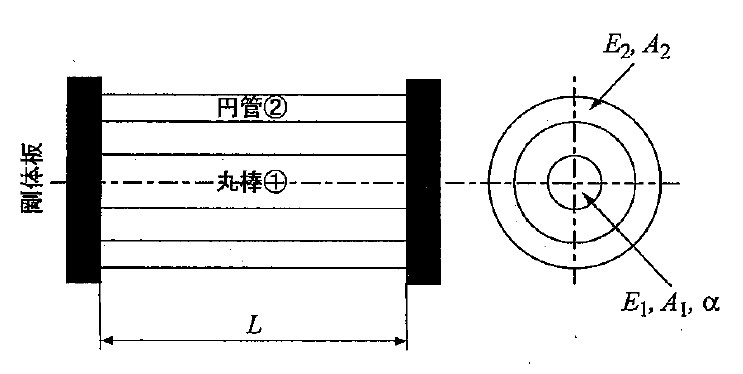
\includegraphics[width=120mm]{images/zairiki_image4.jpg}
        \caption{H24 試験問題 [1]}
    \end{center}
\end{figure}
\begin{enumerate}[(1)]
    \item \textgt{丸棒1に生じるひずみ$\varepsilon_1$を求める}
          \begin{itembox}[l]{Point}
              \begin{center}
                  材料が温度$\Delta T$だけ上昇すると,ひずみに$\alpha \Delta T$が追加される\\
                  (\textgt{合計のひずみ} $\varepsilon'$) = (\textgt{温度上昇によるひずみ} $\alpha \Delta T$) + (\textgt{応力(外力)によるひずみ} $\varepsilon$ )
              \end{center}
          \end{itembox}
          ここで,熱ひずみ$\varepsilon_T$は温度$T$だけ上昇したとき,
          \begin{eqnarray*}
              \varepsilon_T=\alpha T
          \end{eqnarray*}
          また,応力によるひずみ$\varepsilon_\sigma$は
          \begin{eqnarray*}
              \varepsilon_\sigma=\frac{\sigma_1}{E_1}
          \end{eqnarray*}
          したがって,丸棒1のひずみ$\varepsilon_1$は
          \begin{eqnarray*}
              \varepsilon_1&=&\varepsilon_T+\varepsilon_\sigma\\
              &=&\alpha T+\dfrac{\sigma_1}{E_1}
          \end{eqnarray*}
    \item \textgt{丸棒1に生じる応力$\sigma_1$を求める}\\
          \begin{itembox}[l]{Point}
              \begin{center}
                  $\sigma_2$を$\sigma_1$を用いた式で表す
              \end{center}
          \end{itembox}
          力のつり合いより,
          \begin{eqnarray*}
              \sigma_1A_1+\sigma_2A_2=0
          \end{eqnarray*}
          また,伸びは合わせて丸棒1の熱膨張分であるので,
          \begin{eqnarray*}
              \lambda_1+\lambda_2&=&0\\
              \lambda_1&=&-\lambda_2
          \end{eqnarray*}
          両辺を丸棒1,円管2の長さ$L$で割ると,ひずみのつり合いとなる.
          \begin{eqnarray*}
              \frac{\lambda_1}{L}&=&-\frac{\lambda_2}{L}\\
              \varepsilon_1&=&-\varepsilon_2
          \end{eqnarray*}
          したがって,
          \begin{eqnarray*}
              \varepsilon_2&=&-\varepsilon_1=-\left(\alpha T+\dfrac{\sigma_1}{E_1}\right)\\
              \sigma_2&=&E_2\varepsilon_2=-E_2\left(\alpha T+\dfrac{\sigma_1}{E_1}\right)
          \end{eqnarray*}
          これを,力のつり合いの式に代入して整理すると
          \begin{eqnarray*}
              \sigma_1=-\frac{E_1E_2A_2\alpha T}{E_1A_1+E_2A_2}
          \end{eqnarray*}
\end{enumerate}
\subsection{SFDとBMD}
\subsubsection{せん断力線図(SFD)}
はりにはたらくせん断力を図で表したもの
\subsubsection{曲げ応力線図(BMD)}
\begin{itembox}[l]{Point}
    \begin{itemize}
        \item
    \end{itemize}
\end{itembox}
はりにはたらく曲げモーメントを図で表したもの
\subsubsection{(例題) BMDとSFDを書く}

\subsection{不静定問題}
\begin{itembox}[l]{条件}
    \begin{enumerate}[(1)]
        \item 力・トルクのつり合い
        \item 伸び・ねじれ角のつり合い
    \end{enumerate}
\end{itembox}
\begin{itembox}[l]{Point}
    \begin{center}
        \textgt{力・トルク}のつり合いから\textgt{伸び・ねじれ角}を含む式に変換する
    \end{center}
\end{itembox}
\subsubsection{(例題) 不静定問題を解く}
\begin{figure}[htbp]
    \begin{center}
        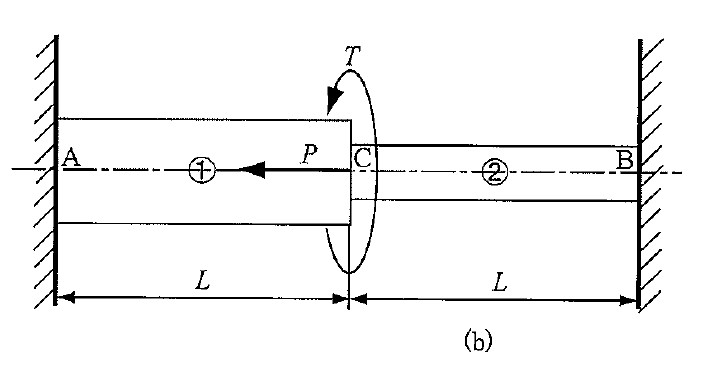
\includegraphics[width=120mm]{images/zairiki_image3.jpg}
        \caption{H27 試験問題 [1]}
    \end{center}
\end{figure}
\begin{enumerate}[(1)]
    \item \textgt{$x=L$に荷重$P$が加わっているときの丸棒2の伸び$\lambda_2$を求める.}\\
          \\
          力のつり合いより,
          \begin{eqnarray*}
              \sigma_1A_1+\sigma_2A_2=P
          \end{eqnarray*}
          伸びは合計でゼロになるので,
          \begin{eqnarray*}
              \lambda_1+\lambda_2&=&0\\
              \lambda_1&=&-\lambda_2
          \end{eqnarray*}
          ここで,応力$\sigma_1,\sigma_2$は,伸び$\lambda_1,\lambda_2$を用いて
          \begin{eqnarray*}
              \sigma_1&=&E\frac{\lambda_1}{L}\\
              \sigma_2&=&E\frac{\lambda_2}{L}
          \end{eqnarray*}
          と表せることから,力のつり合い式に代入すると,
          \begin{eqnarray*}
              E\frac{\lambda_2}{L}A_1+E\frac{\lambda_2}{L}A_2=P
          \end{eqnarray*}
          したがって,
          \begin{eqnarray*}
              \frac{E}{L}\left(\lambda_1A_1+\lambda_2A_2\right)&=&P\\
              \frac{E}{L}\lambda_2\left(A_2-A_1\right)&=&P\\
              \lambda_1&=&\frac{PL}{E\left(A_2-A_1\right)}
          \end{eqnarray*}\\
    \item \textgt{$x=L$にトルク$T$が加わっているときの丸棒2のねじれ角$\varphi_2$を求める.}\\
          \\
          トルクのつり合いより,
          \begin{eqnarray*}
              T_1+T_2=T
          \end{eqnarray*}
          ねじり角は合わせてゼロになるので,
          \begin{eqnarray*}
              \varphi_1+\varphi_2&=&0\\
              \varphi_1&=&-\varphi_2
          \end{eqnarray*}
          ここで,トルク$T_1,T_2$はねじれ角$\varphi_1,\varphi_2$を用いて,
          \begin{eqnarray*}
              T_1&=&I_{P1}G\frac{\varphi_1}{L}\\
              T_2&=&I_{P1}G\frac{\varphi_2}{L}\\
          \end{eqnarray*}
          と表せることから,トルクのつり合い式に代入すると,
          \begin{eqnarray*}
              I_{P1}G\frac{\varphi_1}{L}+I_{P2}G\frac{\varphi_2}{L}=T
          \end{eqnarray*}
          したがって,
          \begin{eqnarray*}
              \frac{G}{L}\left(I_{P1}\varphi_1+I_{P2}\varphi_2\right)&=&T\\
              \frac{G}{L}\varphi_2\left(I_{P2}-I_{P1}\right)&=&T\\
              \varphi_2&=&\frac{TL}{G\left(I_{P2}-I_{P1}\right)}
          \end{eqnarray*}
\end{enumerate}
\subsection{モールの応力円}
\subsection{材料の破断}
塑性変形するときは金属材料が単軸応力状態で変形することはなく,2軸または3軸の応力を受けている.
このような組合せ応力のもとにおいて金属材料が弾性限度に達し,
塑性変形を開始するときの条件を降伏条件という.\\
$\sigma_Y$を材料の降伏強度として代表的な降伏条件式を以下に示す.
\subsubsection{最大主応力説}
この破損則は脆性材料に一致することが多い.
\begin{itembox}[l]{最大主応力説}
    \begin{eqnarray*}
        \sigma_1\geq\sigma_Y\\
    \end{eqnarray*}
\end{itembox}
\subsubsection{最大せん断応力説}
この破損則は,延性材料に一致することが多い.Trescaの説とも呼ばれる.
\begin{itembox}[l]{最大せん断応力説}
    \begin{eqnarray*}
        \dfrac{\sigma_1-\sigma_3}{2}\geq\dfrac{\sigma_Y}{2}\\
    \end{eqnarray*}
\end{itembox}
\subsubsection{せん断ひずみエネルギー説}
この破損則は,延性材料に一致することが多い.Von-Misesの説とも呼ばれる.
\begin{itembox}[l]{せん断ひずみエネルギー説}
    \begin{eqnarray*}
        \dfrac{1}{2}\left[\left(\sigma_3-\sigma_1\right)^2+\left(\sigma_1-\sigma_2\right)^2+\left(\sigma_2-\sigma_3\right)^2\right]\geq\left(\sigma_Y\right)^2\\
    \end{eqnarray*}
\end{itembox}
\subsection{薄肉円筒}
\begin{figure}[htbp]
    \begin{center}
        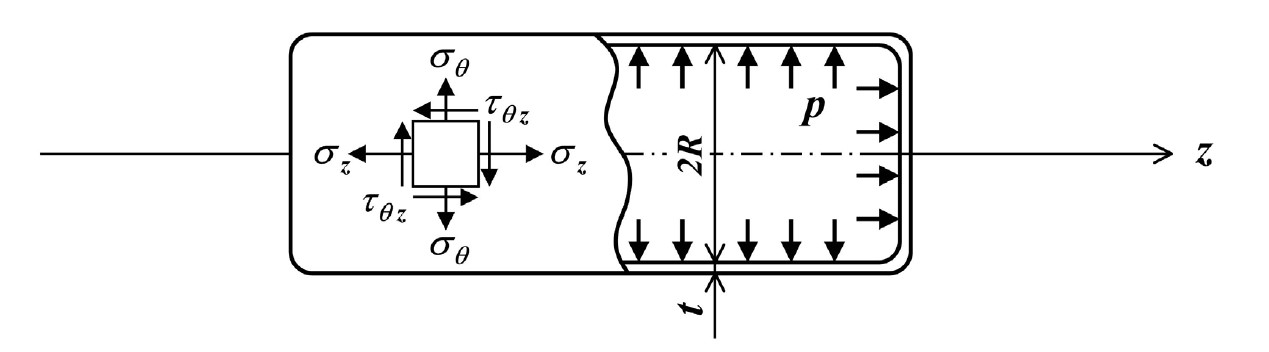
\includegraphics[width=150mm]{images/zairiki_image1.jpg}
        \caption{材料力学2 講義資料1}
    \end{center}
\end{figure}
薄肉とは,上図の内半径$R$に比べて,板厚$t$が十分に小さい,すなわち$t/R \geqq 0.1$のとき程度の場合を指す.\\
このとき,以下の近似が成り立つものとする.
\begin{enumerate}[(1)]
    \item 半径方向応力$\sigma_r$は無視できる
    \item 周方向応力$\sigma_\theta$は板厚に沿って一様である
\end{enumerate}
\subsubsection{それぞれの応力を求める}
周方向応力$\sigma_r$は近似が成立することから,
\begin{eqnarray*}
    \sigma_r=0
\end{eqnarray*}
\begin{figure}[htbp]
    \begin{center}
        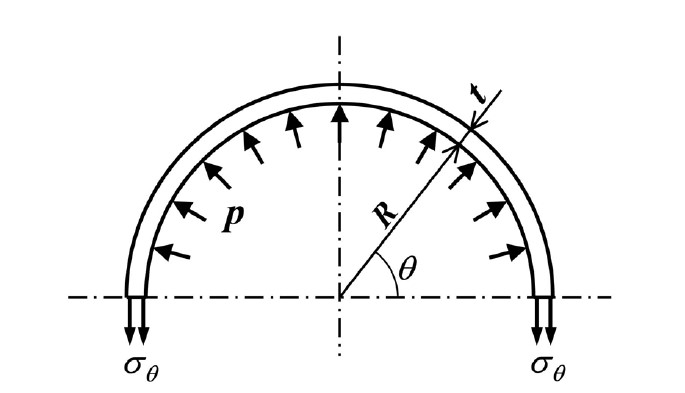
\includegraphics[width=100mm]{images/zairiki_image2.jpg}
        \caption{材料力学2 講義資料2}
    \end{center}
\end{figure}
上図は,円筒を切断したものであり,図の上下方向の力のつり合いより,周方向応力$\sigma_\theta$は,
\begin{eqnarray*}
    \displaystyle
    2t\sigma_\theta &=& \int^\pi_0 pR\sin\theta d\theta = 2pR\\
    \sigma_\theta &=&\dfrac{pr}{t}
\end{eqnarray*}
また,軸方向応力$\sigma_z$は$z$方向の力のつり合いより,
\begin{eqnarray*}
    2\pi Rt \sigma_z&=& \pi R^2p\\
    \sigma_z&=&\dfrac{pr}{2t}
\end{eqnarray*}
したがって,内圧$p$を受ける薄肉円筒に加わる応力は,
\begin{itembox}[l]{薄肉円筒に働く応力}
    \begin{eqnarray*}
        \sigma_r=0\quad
        \sigma_\theta =\dfrac{pr}{t}\quad
        \sigma_z=\dfrac{pr}{2t}
    \end{eqnarray*}
\end{itembox}
なお,外力として荷重$Q$とトルク$T$を受けている場合は,
以上の円筒に生じる応力に,荷重$Q$による垂直応力とトルク$T$によるせん断応力を加えれば良い.
\newpage
\section{機械力学}
\subsection{一自由度並進運動}
\begin{itembox}[l]{運動方程式}
    \begin{eqnarray*}
        m\ddot{x}\left(t\right)+c\dot{x}\left(t\right)+kx\left(t\right)=F\left(t\right)\\
    \end{eqnarray*}
\end{itembox}
\subsection{剛体円盤のねじり振動系}
\begin{itembox}[l]{運動方程式}
    \begin{eqnarray*}
        I\ddot{\theta}\left(t\right)+c_\theta\dot{\theta}\left(t\right)+k_\theta\theta\left(t\right)&=&M\left(t\right)\\
    \end{eqnarray*}
\end{itembox}
\subsection{(例題) 回転に関する運動方程式を求める}
\begin{figure}[htbp]
    \begin{center}
        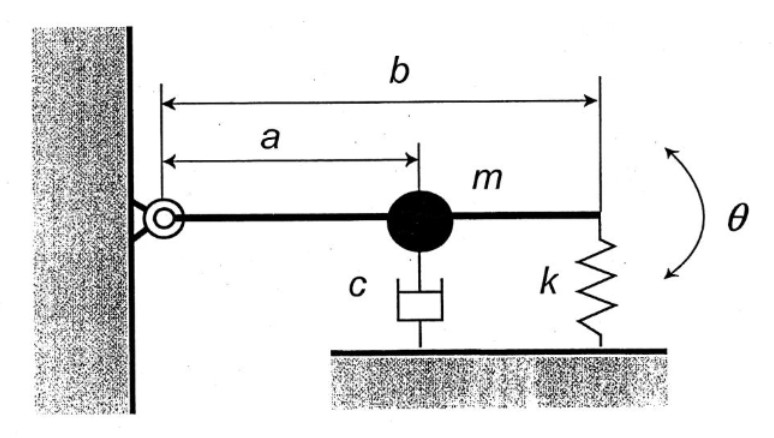
\includegraphics[width=100mm]{images/kiriki_image2.jpg}
        \caption{H18 試験問題 [3]}
    \end{center}
\end{figure}
\begin{itembox}[l]{Point}
    \begin{center}
        \textgt{(モーメント) = (発生する力) $\times$ (腕の長さ)}\\
        運動方程式に\textgt{腕の長さの二乗}が項に出てくる
    \end{center}
\end{itembox}
\begin{enumerate}[(1)]
    \item 質点について\\
          \begin{eqnarray*}
              (質点にはたらくモーメント)&=& [質点にはたらく力] \times (腕の長さ)\\
              &=& [(質量) \times (腕の長さ) \times (角加速度)] \times (腕の長さ)\\
              &=& m \times a \times \ddot{\theta}\left(t\right) \times a\\
              &=&ma^2\ddot{\theta}\left(t\right)
          \end{eqnarray*}
    \item ダッシュポットについて
          \begin{eqnarray*}
              (ダッシュポットにはたらくモーメント)&=& [ダッシュポットにはたらく力] \times (腕の長さ)\\
              &=& [(減衰係数) \times (腕の長さ) \times (角速度)] \times (腕の長さ)\\
              &=& m \times a \times \dot{\theta}\left(t\right) \times a\\
              &=&ca^2\dot{\theta}\left(t\right)
          \end{eqnarray*}
    \item ばねについて
          \begin{eqnarray*}
              (ばねにはたらくモーメント)&=& [ばねにはたらく力] \times (腕の長さ)\\
              &=& [(ばね定数)) \times (腕の長さ) \times (回転角)] \times (腕の長さ)\\
              &=& m \times b \times \theta\left(t\right) \times b\\
              &=&kb^2\dot{\theta}\left(t\right)
          \end{eqnarray*}
\end{enumerate}
以上の(1),(2),(3)より,回転に関する運動方程式は
\begin{eqnarray*}
    ma^2\ddot{\theta}\left(t\right)+ca^2\dot{\theta}\left(t\right)+kb^2\dot{\theta}\left(t\right)=0\\
\end{eqnarray*}
\subsection{自由振動}
外力がゼロのとき,自由振動という.\\
このとき,運動方程式の右辺はゼロとなり,そのときの応答は2階の同次微分方程式を解くことで求めることができる.
\begin{itembox}[l]{Point}
    \begin{eqnarray*}
        (固有振動数\;\omega)&=&(減衰のない系の自由振動の振動数)\\
        (減衰固有振動数\;\omega_d)&=&(減衰のある系の自由振動の振動数(減衰自由振動数))\\
    \end{eqnarray*}
\end{itembox}
\begin{itembox}[l]{固有振動数}
    \begin{eqnarray*}
        \omega_n = \sqrt{\dfrac{k}{m}}\\
    \end{eqnarray*}
\end{itembox}
\begin{itembox}[l]{減衰比}
    \begin{eqnarray*}
        \zeta = \dfrac{c}{2\sqrt{mk}}\\
    \end{eqnarray*}
\end{itembox}
\begin{itembox}[l]{減衰固有振動数}
    \begin{eqnarray*}
        \omega_d&=&\sqrt{1-\zeta^2}\omega_n\\
    \end{eqnarray*}
\end{itembox}
\begin{itembox}[l]{振動数と周期}
    \begin{eqnarray*}
        \omega=\dfrac{2\pi}{T}\\
    \end{eqnarray*}
\end{itembox}
\subsection{特性方程式}
運動方程式(自由振動)に$\; x\left(x\right)=e^{st}\;$を代入して整理すると,以下のような\textgt{特性方程式}を得ることができる.
\begin{itembox}[l]{特性方程式}
    \begin{eqnarray*}
        s^2+2\zeta\omega_ns+\omega_n^2=0\\
    \end{eqnarray*}
\end{itembox}
これを満たす$\; s_1,s_2\;$の組を\textgt{特性根}という.
\subsubsection{過減衰}
$\zeta>1$のとき,特性根は
\begin{eqnarray*}
    s_1,s_2=\left(-\zeta \pm \sqrt{\zeta^2-1}\right)\omega_n
\end{eqnarray*}
の相異なる負の実数となる.
したがって,応答$x\left(t\right)$は以下のようになる.
\begin{itembox}[l]{過減衰の応答}
    \begin{eqnarray*}
        x\left(t\right)=a_1\exp{\left(s_1t\right)}+a_2\exp{\left(s_2t\right)}\\
    \end{eqnarray*}
\end{itembox}
ここで,$t\rightarrow\infty$で$0$に漸近する.
そのため,振動は繰り返しを伴わない.($\neq$振動)\\
このとき,これを\textgt{過減衰}という.
\subsubsection{臨界減衰}
$\zeta = 0$のとき,特性根は
\begin{eqnarray*}
    s_1=s_2=-\omega_n
\end{eqnarray*}
したがって,応答$x\left(t\right)$は以下のようになる.
\begin{itembox}[l]{臨界減衰の応答}
    \begin{eqnarray*}
        x\left(t\right)=a_1\exp{\left(-\omega_nt\right)}+a_2t\exp{\left(-\omega_nt\right)}\\
    \end{eqnarray*}
\end{itembox}
このときの応答を\textgt{臨界減衰}といい,応答の収束が最も速くなる.
\subsubsection{不足減衰}
$0<\zeta<1$のとき,特性根は
\begin{eqnarray*}
    s_1,s_2=\left(-\zeta \pm i\sqrt{1-\zeta^2}\right)\omega_n\\
\end{eqnarray*}
の共役な複素数となる.
したがって,応答$x\left(t\right)$は以下のようになる.(導出省略)
\begin{itembox}[l]{不足減衰の応答}
    \begin{eqnarray*}
        x\left(t\right)&=&A\exp{\left(-\zeta \omega_nt\right)}\cos{\left(\sqrt{1-\zeta^2}\omega_nt\right)}+B\exp{\left(-\zeta \omega_nt\right)}\sin{\left(\sqrt{1-\zeta^2}\omega_nt\right)}\\
        x\left(t\right)&=&A\exp{\left(-\zeta \omega_nt\right)}\cos{\left(\omega_dt\right)}+B\exp{\left(-\zeta \omega_nt\right)}\sin{\left(\omega_dt\right)}\\
        \\
        x\left(t\right)&=&C\exp{\left(-\zeta \omega_nt\right)}\cos\left(\sqrt{1-\zeta^2}\omega_nt+\varphi\right)
    \end{eqnarray*}
    \begin{eqnarray*}
        \omega_d=\sqrt{1-\zeta^2}\omega_n\;&:&\;減衰固有振動数\\
        \varphi\;&:&\;位相角\\
        ※ A,B,C&&は任意定数\\
    \end{eqnarray*}
\end{itembox}
\begin{itembox}[l]{三角関数の合成}
    \begin{eqnarray*}
        a\sin\theta+b\cos\theta
        &=&\sqrt{a^2+b^2}\left(\dfrac{a}{\sqrt{a^2+b^2}}\sin\theta+\dfrac{b}{\sqrt{a^2+b^2}}\cos\theta\right)\\
        &=&\sqrt{a^2+b^2}\left(\sin\theta\dfrac{a}{\sqrt{a^2+b^2}}+\cos\theta\dfrac{b}{\sqrt{a^2+b^2}}\right)\\
        &=&\sqrt{a^2+b^2}\left(\sin\theta\cos\alpha+\cos\theta\sin\alpha\right)\\
        &=&\sqrt{a^2+b^2}\sin\left(\theta+\alpha\right)\\
        \\
        a\sin\theta+b\cos\theta
        &=&\sqrt{a^2+b^2}\left(\dfrac{a}{\sqrt{a^2+b^2}}\sin\theta+\dfrac{b}{\sqrt{a^2+b^2}}\cos\theta\right)\\
        &=&\sqrt{a^2+b^2}\left(\cos\theta\dfrac{b}{\sqrt{a^2+b^2}}+\sin\theta\dfrac{a}{\sqrt{a^2+b^2}}\right)\\
        &=&\sqrt{a^2+b^2}\left(\cos\theta\cos\alpha+\sin\theta\sin\alpha\right)\\
        &=&\sqrt{a^2+b^2}\cos\left(\theta-\alpha\right)\\
        \\
        ※\quad\tan\alpha &=& -\dfrac{b}{a}
    \end{eqnarray*}
\end{itembox}
\subsubsection{単振動}
$\zeta = 0$のとき,特性根は
\begin{eqnarray*}
    s_1,s_2=i\omega_n\\
\end{eqnarray*}
の共役な純虚数となる.
したがって,応答$x\left(t\right)$は以下のようになる.(導出省略)
\begin{itembox}[l]{単振動の応答}
    \begin{eqnarray*}
        x\left(t\right)&=&A\cos{\omega_nt}+B\sin{\omega_nt}\\
    \end{eqnarray*}
\end{itembox}
このとき,減衰係数$\zeta=0$より,いつまでも減衰しない\textgt{単振動}となる.\\
\\
ここで,極の実部(負になる)は\textgt{自由振動の減衰の速さ}を表し,極の虚部は\textgt{自由振動の振動数}を表している.
\subsection{強制振動}
\textgt{強制振動}とは,外力が存在する振動である.\\
このとき,運動方程式の右辺に外力$f\left(t\right)$の項を持ち,その応答は
重ね合わせの原理から右辺がゼロの自由振動における2階の同次微分方程式の一般解に,
特殊解を足し合わせることで求めることができる.\\
\subsection{調和外力に対する定常応答}
\begin{itembox}[l]{調和外力}
    \begin{center}
        周期性を持つ外力のことを\textgt{調和外力}という.$\sin$波や$\cos$波に相当する.
    \end{center}
\end{itembox}
\begin{itembox}[l]{定常応答}
    \begin{center}
        加振開始から十分な時間が経過した後の応答を\textgt{定常応答}といい,運動方程式の\textgt{特殊解}に相当する.\\
        また,そのような状況を\textgt{定常状態}という.定常応答解析では初期時刻という概念を考えない.\\
        外力は無限の過去に始まり,未来永劫続いている
    \end{center}
\end{itembox}
\subsubsection{三角関数による方法}
定常応答を求めるには,
\begin{eqnarray*}
    m \ddot{x}\left(t\right)+c\dot{x}\left(t\right)+kx\left(t\right)=f\cos\omega t
\end{eqnarray*}
を解けばよい.(ここでは,外力を$f\left(t\right)=f\cos\omega t$)としている.\\
外力$f\left(t\right)$が\textgt{振動数$\omega$をもつ繰り返し力}であることから,
それに駆動される定常応答もまた\textgt{同じ振動数を持つ繰り返し}になるはずである.
ただし,\textgt{振幅}(振動の大きさ)と\textgt{位相}(山谷のタイミング)は異なる可能性がある.\\
ここで,振幅$x_0$と外力に対する位相遅れ$\varphi$を未知量として,特殊解の形を$x\left(t\right)=x_0\cos\left(\omega t-\varphi\right)$
と\textgt{予想する}して,運動方程式に代入し$\cos\varphi,\sin\varphi$について整理すると
\begin{eqnarray*}
    x_0\cos\varphi&=&\dfrac{-m\omega^2+k}{\left(-m\omega^2+k\right)^2+\left(c\omega\right)^2}f\\
    x_0\sin\varphi&=&\dfrac{c\omega}{\left(-m\omega^2+k\right)^2+\left(c\omega\right)^2}f
\end{eqnarray*}
したがって,振幅$x_0$は,
\begin{itembox}[l]{振幅$x_0$}
    \begin{eqnarray*}
        x_0=\sqrt{\left(x_0\cos\varphi\right)^2+\left(x_0\sin\varphi\right)^2}=\dfrac{1}{\sqrt{\left(-m\omega^2+k\right)^2+\left(c\omega\right)^2}}f\\
    \end{eqnarray*}
\end{itembox}
位相遅れ$\varphi$は,$x_0\cos\varphi,x_0\sin\varphi$の比をとったものであるので,
\begin{itembox}[l]{位相遅れ$\varphi$}
    \begin{eqnarray*}
        \varphi=\mathrm{Tan}^{-1}\left(\dfrac{x_0\sin\varphi}{x_0\cos\varphi}\right)=\mathrm{Tan}^{-1}\left(\dfrac{c\omega}{-m\omega^2+k}\right)\\
    \end{eqnarray*}
\end{itembox}
\subsubsection{複素振幅表示による方法(1)}
\begin{itembox}[l]{Point}
    \begin{eqnarray*}
        f\left(t\right)
        &=&Fe^{i\omega t}\\
        &=&A\cos\left(\omega t\right)+Bi\sin\left(\omega t\right)\\
        &=&|F|\sin\left(\omega t -\varphi_1\right)\\
        &=&|F|\cos\left(\omega t -\varphi_2\right)\\
        \\
        f\left(t\right) &が& \sin\; の項を持つ場合\; \rightarrow \; A=0\\
        f\left(t\right) &が& \cos\; の項を持つ場合\; \rightarrow \; B=0\\
    \end{eqnarray*}
\end{itembox}
三角関数を用いて考えたときと同様に外力を$f\left(t\right)=f\cos\omega t$とする.
\begin{eqnarray*}
    x\left(t\right)&=&Xe^{i\omega t}\\
    f\left(t\right)&=&Fe^{i\omega t}\\
    ※\quad\omega &:& 外力の振動数
\end{eqnarray*}
を代入することで,三角関数を用いる方法より簡単に応答の振幅,位相遅れを求めることができる.\\
ここで,$X$を\textgt{複素振幅}といい,$|X|$は\textgt{振動振幅}$x_0$を,
$-\angle X$は\textgt{位相遅れ}$\varphi$を表す.\\
\begin{itembox}[l]{Point}
    \begin{center}
        \textgt{複素振幅}を用いることで,\textgt{振動振幅}と\textgt{位相遅れ}の2つの情報を1つの関数で表すことができる
    \end{center}
\end{itembox}
以上の式を,運動方程式に代入して整理すると,\\
\begin{eqnarray*}
    \left(-m\omega^2+ic\omega+k\right)Xe^{i\omega t}=Fe^{i\omega t}\\
\end{eqnarray*}
となることから,複素振幅$X$,振動振幅$|X|$,位相遅れ$\varphi$は,
\begin{itembox}[l]{複素振幅$X$}
    \begin{eqnarray*}
        X=\dfrac{F}{-m\omega^2+ic\omega+k}\\
    \end{eqnarray*}
\end{itembox}
\begin{itembox}[l]{振動振幅$|X|$}
    \begin{eqnarray*}
        x_0=|X|&=&\dfrac{F}{\sqrt{\left(-m\omega^2+k\right)^2+\left(c\omega\right)^2}}\\
    \end{eqnarray*}
\end{itembox}
\begin{itembox}[l]{位相遅れ$\varphi$}
    \begin{eqnarray*}
        \varphi=-\angle X &=&\mathrm{Tan}^{-1}\left(\dfrac{c\omega}{-m\omega^2+k}\right)\\
    \end{eqnarray*}
\end{itembox}
定常応答$x\left(t\right)$は,
\begin{eqnarray*}
    x\left(t\right)&=&x_0\cos\left(\omega t-\varphi\right)\\
\end{eqnarray*}
に上記の値を代入したものになる.\\
\subsubsection{複素振幅表示による方法(2)}
つぎに,固有振動数$\omega_n$,減衰比$\zeta$を用いて考える.\\
このとき,運動方程式は以下のように書き換えることができる.
\begin{eqnarray*}
    \ddot{x}\left(t\right)+2\zeta\omega_n\dot{x}\left(t\right)+\omega_n^2 x\left(t\right)=\frac{f}{m}\cos\omega t
\end{eqnarray*}
同様に,以下の式を運動方程式に代入して整理すると,
\begin{eqnarray*}
    x\left(t\right)&=&Xe^{i\omega t}\\
    f\left(t\right)&=&Fe^{i\omega t}\\
    ※\quad\omega &:& 外力の振動数\\
    ※\quad F &=& \frac{f}{m}
\end{eqnarray*}
\begin{eqnarray*}
    \left(-\omega^2+2\zeta\omega_n\omega i+\omega_n^2\right)Xe^{i\omega t}=Fe^{i\omega t}\\
\end{eqnarray*}
となることから,複素振幅$X$,振動振幅$|X|$,位相遅れ$\varphi$は,
\begin{itembox}[l]{複素振幅$X$}
    \begin{eqnarray*}
        X=\dfrac{F}{-\omega^2+2\zeta\omega_n\omega i+\omega_n^2}\\
    \end{eqnarray*}
\end{itembox}
\begin{itembox}[l]{振動振幅$|X|$}
    \begin{eqnarray*}
        x_0=|X|&=&\dfrac{F}{\sqrt{\left(\omega_n^2-\omega^2\right)^2+\left(2\zeta\omega_n\omega\right)^2}}\\
    \end{eqnarray*}
\end{itembox}
\begin{itembox}[l]{位相遅れ$\varphi$}
    \begin{eqnarray*}
        \varphi=-\angle X &=&\mathrm{Tan}^{-1}\left(\dfrac{2\zeta\omega_n\omega}{\omega_n^2-\omega^2}\right)\\
    \end{eqnarray*}
\end{itembox}
定常応答$x\left(t\right)$は,
\begin{eqnarray*}
    x\left(t\right)&=&x_0\cos\left(\omega t-\varphi\right)\\
\end{eqnarray*}
に上記の値を代入したものになる.\\
※ 調和振動が $\sin$ の項を持つ場合は,$\cos$から$\sin$に変えれば良い.
\subsubsection{周波数応答関数$G_f$}
$X/F$の絶対値は外力の振幅に対する応答の\textgt{振幅比}を,偏角に負号をつけたものは外力に対する応答の位相遅れを表す.
ここで,$G_f=X/F$とおくと,$G_f$は$\omega$の関数になり,これを\textgt{周波数応答関数}という.
\begin{itembox}[l]{周波数応答関数}
    \begin{eqnarray*}
        G_f\left(\omega\right)=\dfrac{X}{F}=\dfrac{1}{-m\omega^2+ic\omega +k}\\
    \end{eqnarray*}
\end{itembox}
周波応答関数は,\textgt{単位大きさの正弦波外力に対する定常応答の複素振幅}を,\textgt{外力の振動数(加振振動数)}の関数としてあらわしたものである.
\begin{itembox}[l]{振幅比$|X/F|$}
    \begin{eqnarray*}
        \left|\dfrac{X}{F}\right|=|G_f\left(\omega\right)|=\dfrac{1}{-m\omega^2+ic\omega+k}\\
    \end{eqnarray*}
\end{itembox}
\begin{itembox}[l]{位相遅れ$\varphi$}
    \begin{eqnarray*}
        \varphi=-\angle X &=&\tan^{-1}\left(\dfrac{c\omega}{-m\omega^2+k}\right)\\
    \end{eqnarray*}
    \begin{center}
        ※ 複素振幅の位相遅れと同じ
    \end{center}
\end{itembox}
\subsection{共振曲線}

\subsection{その他}
\subsubsection{合成ばね定数を求める}
系の平衡状態から,力を加えたと仮定して力のつり合いを考えることで合成ばね定数を求めることができる.
\begin{itembox}[l]{Point}
    \begin{center}
        (\textgt{質点に加わる力})\quad=\quad(\textgt{合成ばね定数})\quad×\quad(\textgt{変位の合計})
    \end{center}
\end{itembox}
※ 質点に加わる力は,「$f$」等で適当におくと良い.(後々消える)
\newpage
\section{熱力学}
\subsection{熱力学第一法則}
\begin{screen}
    \begin{center}
        \textgt{熱}と\textgt{仕事}は本質的に同種のエネルギーであり,それらは互いに\textgt{変換可能}である
    \end{center}
\end{screen}
\subsubsection{閉じた系}
物質の出入りのない系のことを\textgt{閉じた系}という.\quad 例) ピストン-シリンダ系
\begin{itembox}[l]{閉じた系の熱力学第一法則}
    \begin{eqnarray*}
        Q&=&\Delta U+W\\
        Q&:&受熱量\\
        \Delta U&:&内部エネルギの変化量\\
        W&:&絶対仕事\\
    \end{eqnarray*}
\end{itembox}
\subsubsection{内部エネルギ}
個々の分子は力学的エネルギ(位置エネルギ+運動エネルギ)を持っている。\\
それを巨視的に見たときに分子の持つ\textgt{内部エネルギ}と呼ぶ。
\begin{itembox}[l]{内部エネルギの変化量}
    \begin{eqnarray*}
        \Delta U&=&mC_v\Delta T\\
    \end{eqnarray*}
\end{itembox}
初期状態を$\left(P,v,T\right)$とする.\\
※ $v$は比容積
\subsubsection{開いた系}
物質の出入りがある系のことを\textgt{開いた系}という.\quad 例) タービン\\
また,このとき取り出される仕事を\textgt{工業仕事}という.
\begin{itembox}[l]{開いた系の熱力学第一法則}
    \begin{eqnarray*}
        Q&=&\Delta H+W_t\\
        Q&:&受熱量\\
        \Delta H&:&エンタルピの変化量\\
        W_t&:&工業仕事\\
    \end{eqnarray*}
\end{itembox}
\subsubsection{エンタルピ}
内部エネルギーと流動エネルギを合わせたものをエンタルピと定義される。
\begin{itembox}[l]{Point}
    \begin{center}
        閉じた系における\textgt{等圧過程での受熱量(放熱量)}のこと!!
    \end{center}
\end{itembox}
\begin{itembox}[l]{エンタルピ}
    \begin{eqnarray*}
        H=U+W\\
    \end{eqnarray*}
\end{itembox}
\begin{itembox}[l]{エンタルピの変化量}
    \begin{eqnarray*}
        \Delta H&=&mC_p\Delta T\\
    \end{eqnarray*}
\end{itembox}
\subsection{理想気体}
\begin{itembox}[l]{状態方程式}
    \begin{eqnarray*}
        PV&=&mRT\\
        Pv&=&RT\quad (単位質量基準の場合)\\
        ※v&:&比容積\\
    \end{eqnarray*}
\end{itembox}
\begin{itembox}[l]{マイヤーの法則}
    \begin{eqnarray*}
        C_p&=&C_v+R\\
        C_p&:&定圧比熱\\
        C_v&:&定容比熱\\
    \end{eqnarray*}
\end{itembox}
\subsection{熱力学第二法則}
\begin{screen}
    \begin{center}
        熱は高いほうから低いほうへと移動するという\textgt{不可逆現象}のことを指す.
    \end{center}
\end{screen}
\subsubsection{仕事}
\begin{itembox}[l]{仕事}
    \begin{eqnarray*}
        W&=&Q_H-Q_L\\
        W&=&\displaystyle \int PdV\quad(閉じた系の絶対仕事)\\
        W_t&=&\displaystyle \int VdP\quad(開いた系の工業仕事) \\
    \end{eqnarray*}
\end{itembox}
\begin{itembox}[l]{正味の仕事}
    \begin{eqnarray*}
        W_{net} &=& (膨張過程で\;\textgt{した仕事}) - (圧縮過程で\;\textgt{された仕事})\\
        &=& (膨張過程で\;\textgt{した仕事}) + (圧縮過程で\;\textgt{した仕事})\\
        &=& (膨張過程で\;\textgt{された仕事}) + (圧縮過程で\;\textgt{された仕事})\\
    \end{eqnarray*}
\end{itembox}
\subsubsection{熱効率}
\begin{itembox}[l]{熱効率}
    \begin{eqnarray*}
        \eta_{th}=\dfrac{W}{Q_H}=1-\dfrac{Q_L}{Q_H}\\
    \end{eqnarray*}
\end{itembox}
\subsection{エントロピ}
2つの状態間を\textgt{不可逆的に変化}させたとき,
その変化の経路に無関係に一定となる値(\textgt{状態量})のこと.\\
また,その変化の不可逆性の大きさを示す.可逆断熱過程では,エントロピーの変化は\textgt{ゼロ}になる.
\begin{itembox}[l]{エントロピ}
    \begin{eqnarray*}
        \displaystyle\int \frac{dQ}{T}=const\\
    \end{eqnarray*}
\end{itembox}
\subsection{過程}
\subsubsection{等温過程}
\begin{itembox}[l]{Point}
    \begin{eqnarray*}
        PV&=&const\\
        Q&=&W\\
        \Delta S
        &=& \int \frac{dQ}{T}\\
        &=& \frac{1}{T}\int Pdv\;(閉じた系)\\
        &=& \frac{1}{T}\int Vdp\;(開いた系)\\
    \end{eqnarray*}
\end{itembox}
\subsubsection{等容過程}
\begin{itembox}[l]{Point}
    \begin{eqnarray*}
        \frac{P}{T}&=&const\\
        Q&=&\Delta U = mC_v\Delta T\\
        \\
        \Delta s&=&\int \frac{dQ}{T} = \int \frac{dU}{T} = C_v\int\frac{1}{T}dT\\
    \end{eqnarray*}
\end{itembox}
\subsubsection{等圧過程}
\begin{itembox}[l]{Point}
    \begin{eqnarray*}
        \frac{V}{T}&=&const\\
        Q&=&\Delta U + W = mC_p\Delta T \; \left(= \Delta H\right)\\
        \\
        \Delta s&=&\int \frac{dQ}{T} = \int \frac{dH}{T} = C_p\int\frac{1}{T}dT\\
    \end{eqnarray*}
\end{itembox}
\subsubsection{断熱(等エントロピー)過程}
\begin{itembox}[l]{Point}
    \begin{eqnarray*}
        PV^\kappa&=&const\\
        \Delta U&=&- W\\
        \Delta s&=&0\\
    \end{eqnarray*}
\end{itembox}
\subsubsection*{$PV^\kappa=const$の導出}
熱力学第一法則より、断熱過程では
\begin{eqnarray*}
    0&=&=du+Pdv\\
    &=&C_vdT+PdV
\end{eqnarray*}
理想気体の式$Pv=RT$と比熱の関係式
\subsection{サイクル}
あくまで、理論上のサイクルでありすべて\textgt{閉じた系}と仮定している。
\subsubsection{カルノーサイクル}
\begin{itembox}[l]{過程}
    \begin{center}
        \textgt{(1) 断熱圧縮}\quad → \quad \textgt{(2) 等温膨張} \quad → \quad \textgt{(3) 断熱膨張} \quad → \quad \textgt{(4) 等温収縮}
    \end{center}
\end{itembox}
受熱量をすべて仕事に変換できる等温変化を用いるため,サイクルの中で最も高い熱効率となる.
\begin{itembox}[l]{熱効率}
    \begin{eqnarray*}
        \eta_{thc}=1-\frac{T_2}{T_1}\\
    \end{eqnarray*}
\end{itembox}
\subsubsection{オットーサイクル}
\begin{itembox}[l]{過程}
    \begin{center}
        \textgt{(1) 断熱圧縮}\quad → \quad \textgt{(2) 等容加熱} \quad → \quad \textgt{(3) 断熱膨張} \quad → \quad \textgt{(4) 等容放熱}
    \end{center}
\end{itembox}
\begin{itembox}[l]{圧縮率}
    \begin{eqnarray*}
        \varepsilon=\frac{V_1}{V_2}=\frac{V_3}{V_4}> 1\\
    \end{eqnarray*}
\end{itembox}
\begin{itembox}[l]{熱効率}
    \begin{eqnarray*}
        \eta_{tho}=1-\frac{1}{\varepsilon^{\kappa-1}}\\
    \end{eqnarray*}
\end{itembox}
ガソリンエンジンの基本サイクル.
\subsubsection{ディーゼルサイクル}
\begin{itembox}[l]{過程}
    \begin{center}
        \textgt{(1) 断熱圧縮}\quad → \quad \textgt{(2) 等圧加熱} \quad → \quad \textgt{(3) 断熱膨張} \quad → \quad \textgt{(4) 等容放熱}
    \end{center}
\end{itembox}
\begin{itembox}[l]{締切比 (等圧膨張比)}
    \begin{eqnarray*}
        \sigma=\frac{V_3}{V_2}>1\\
    \end{eqnarray*}
\end{itembox}
ディーゼルエンジンのサイクル.
\subsubsection{サバテサイクル}
\begin{itembox}[l]{過程}
    \begin{center}
        \textgt{(1) 断熱圧縮}\quad → \quad \textgt{(2) 等容加熱}\quad → \quad \textgt{(3) 等圧加熱} \quad → \quad \textgt{($3'$) 断熱膨張} \quad → \quad \textgt{(4) 等容放熱}
    \end{center}
\end{itembox}
\begin{itembox}[l]{圧力比}
    \begin{eqnarray*}
        \alpha=\frac{P_3}{P_2}>1\\
    \end{eqnarray*}
\end{itembox}
高速ディーゼルサイクル.受熱過程が等容変化と等圧変化の組み合わせになっている.
\subsubsection{ブレイトンサイクル}
\begin{itembox}[l]{過程}
    \begin{center}
        \textgt{(1) 断熱圧縮}\quad → \quad \textgt{(2) 等圧加熱} \quad → \quad \textgt{(3) 断熱膨張} \quad → \quad \textgt{(4) 等圧放熱}
    \end{center}
\end{itembox}
ガスタービンやジェットエンジンの基本サイクル.\\
※ 閉じた系と仮定している
\begin{itembox}[l]{断熱効率}
    \begin{eqnarray*}
        \eta &=& \dfrac{h_{2s}-h_1}{h_{2a}-h_1} <1 \quad (圧縮機)\\
        \eta &=& \dfrac{h_3-h_{4a}}{h_3-h_{4s}} <1 \quad (タービン)\\
    \end{eqnarray*}
\end{itembox}
\subsection{再生ブレイトンサイクル}
\subsection{乾き度}
蒸気中の気相部分と液相部分の重量割合のことを\textgt{乾き度}という.\\
$1\mathrm{kg}$の湿り蒸気が$x\mathrm{kg}$の蒸気と$\left(1-x\right)\mathrm{kg}$の液体から成るとき,
$x$を\textgt{乾き度},$\left(1-x\right)$を\textgt{湿り度}という.
\newpage
\section{流体力学}
\subsection{静止流体の力学}
\subsubsection{静水圧}

\subsubsection{表面張力}
液体の分子間には引張合う力がはたらいており,気体やほかの液体と接している面には縮もうとする力が作用する.
これを\textgt{表面張力}といい,単位は$\left[\mathrm{N/m}\right]$である.
\begin{itembox}[l]{Point}
    \begin{center}
        上下方向の力のつり合いを考える\\
    \end{center}
\end{itembox}
\begin{itembox}[l]{表面張力}
    \begin{center}
        表面張力は,\textgt{境界面の接線方向}にはたらく\\
        ( \textgt{液体の重量$\left[\mathrm{N}\right]$} ) = ( \textgt{表面張力の垂直方向成分$\left[\mathrm{N/m}\right]$}) $\times$ ( \textgt{境界面の周の長さ}$\;\left[\mathrm{m}\right]$ )
    \end{center}
\end{itembox}
\subsection{粘性流体の力学}
流体の運動における未知量は,\textgt{速度,圧力,密度,温度}である.\\
また,\textgt{時間$\left(t\right)$,空間$\left(x,y,z\right)$}の関数である.\\
\begin{itembox}[l]{Point}
    \begin{eqnarray*}
        (圧縮性流体)&&\quad 未知量は4つ\quad 速度\left(u,v,w\right),圧力\left(p\right)\\
        (非圧縮性流体)&&\quad 未知量は6つ\quad 速度\left(u,v,w\right),圧力\left(p\right),密度\left(\rho\right),温度\left(T\right)\\
    \end{eqnarray*}
\end{itembox}
\subsection{流体の質量保存則}
\begin{itembox}[l]{連続の式}
    \begin{eqnarray*}
        \dfrac{\partial\rho}{\partial t}+\dfrac{\partial \left(\rho u\right)}{\partial x}+\dfrac{\partial \left(\rho v\right)}{\partial y}+\dfrac{\partial \left(\rho w\right)}{\partial z}&=&0\quad(3次元)\\
        \dfrac{\partial\rho}{\partial t}+\dfrac{\partial \left(\rho u\right)}{\partial x}+\dfrac{\partial \left(\rho v\right)}{\partial y}&=&0\quad(2次元)\\
    \end{eqnarray*}
\end{itembox}
\subsection{流体のエネルギー保存則}
\begin{itembox}[l]{ベルヌーイの定理}
    \begin{eqnarray*}
        \dfrac{1}{2}\dot{m}v^2+\dot{m}\dfrac{p}{\rho}+\dot{m}gz=const\\
    \end{eqnarray*}
\end{itembox}
※ ベルヌーイの定理は,\textgt{エネルギー保存則}であるのでエネルギーの損失 (圧力損失 等) がある場合は適用できない\\
→ 運動量保存則が適用される
\subsubsection{トリチェリの定理}
容器に液体を入れ,容器に対して十分に小さい穴をあける.
このとき,流れが定常であるとすると,流れ出す液体の速度$v$は以下のように表される.
\begin{itembox}[l]{トリチェリの定理}
    \begin{eqnarray*}
        v&=&\sqrt{2gh}\\
        g&:&重力加速度\\
        h&:&水面から穴までの高さ\\
    \end{eqnarray*}
\end{itembox}
これは,ベルヌーイの定理を用いることで証明できる.
\subsection{流体の運動量の法則}
\begin{itembox}[l]{運動量保存則}
    \begin{eqnarray*}
        \displaystyle\sum mv=Ft
    \end{eqnarray*}
    両辺を時間$t$で微分すると,
    \begin{eqnarray*}
        \displaystyle\sum \dot{m}v=F\\
    \end{eqnarray*}
\end{itembox}
\subsection{流体の運動方程式}
\subsubsection{流体の運動を表す2つの運動方程式}
\begin{itembox}[l]{オイラーの運動方程式(2次元)}
    \begin{eqnarray*}
        \dfrac{\partial u}{\partial t}+u\dfrac{\partial u}{\partial x}+v\dfrac{\partial u}{\partial y}&=&-\dfrac{1}{\rho}\dfrac{\partial p}{\partial x}+f_x\quad(x方向)\\
        \dfrac{\partial v}{\partial t}+u\dfrac{\partial v}{\partial x}+v\dfrac{\partial v}{\partial y}&=&-\dfrac{1}{\rho}\dfrac{\partial p}{\partial x}+f_y\quad(y方向)\\
    \end{eqnarray*}
\end{itembox}
\begin{itembox}[l]{ナビエ・ストークス方程式(2次元)\quad(非圧縮性流体)}
    \begin{eqnarray*}
        \dfrac{\partial u}{\partial t}+u\dfrac{\partial u}{\partial x}+v\dfrac{\partial u}{\partial y}&=&-\dfrac{1}{\rho}\dfrac{\partial p}{\partial x}+\nu\left(\dfrac{\partial^2 u}{\partial x^2}+\dfrac{\partial^2 u}{\partial y^2}\right)+f_x\quad(x方向)\\
        \dfrac{\partial v}{\partial t}+u\dfrac{\partial v}{\partial x}+v\dfrac{\partial v}{\partial y}&=&-\dfrac{1}{\rho}\dfrac{\partial p}{\partial y}+\nu\left(\dfrac{\partial^2 v}{\partial x^2}+\dfrac{\partial^2 v}{\partial y^2}\right)+f_y\quad(y方向)\\
        ※\quad \nu &=& \frac{\mu}{\rho} \;:\; 動粘性係数\\
    \end{eqnarray*}
\end{itembox}
\begin{itembox}[l]{ナビエ・ストークス方程式の境界条件}
    \begin{enumerate}
        \item 定常流れ
              \begin{eqnarray*}
                  \dfrac{\partial u}{\partial t}=0
              \end{eqnarray*}
        \item 完全に発達した流れ
              \begin{eqnarray*}
                  \dfrac{\partial u}{\partial x}=0
              \end{eqnarray*}
    \end{enumerate}
\end{itembox}
\begin{itembox}[l]{極座標系の支配方程式\quad(非圧縮性流体)}
    \begin{eqnarray*}
        \dfrac{1}{r}\dfrac{\partial \left(rv_r\right)}{\partial r}+\dfrac{1}{r}\dfrac{\partial v_\theta}{\partial \theta}=0\quad&&(連続の式)\\
        \dfrac{\partial v_r}{\partial t}+v_r\dfrac{\partial v_r}{\partial r}+\dfrac{v_\theta}{r}\dfrac{\partial v_r}{\partial \theta}-\dfrac{{v_\theta}^2}{r}=-\dfrac{1}{\rho}\dfrac{\partial p}{\partial r}+\nu \left(\dfrac{\partial^2 v_r}{\partial r^2}+\dfrac{1}{r}\dfrac{\partial v_r}{\partial r}+\dfrac{1}{r^2}\dfrac{\partial^2 v_r}{\partial \theta^2}-\dfrac{v_r}{r^2}-\dfrac{2}{r^2}\dfrac{\partial v_\theta}{\partial \theta}\right)+f_r\quad&&(r方向)\\
        \dfrac{\partial v_\theta}{\partial t}+v_r\dfrac{\partial v_\theta}{\partial r}+\dfrac{v_\theta}{r}\dfrac{\partial v_\theta}{\partial \theta}+\dfrac{v_rv_\theta}{r}=-\dfrac{1}{\rho}\dfrac{1}{r}\dfrac{\partial p}{\partial \theta}+\nu\left(\dfrac{\partial^2 v_r}{\partial \theta^2}+\dfrac{1}{r}\dfrac{\partial v_\theta}{\partial r}+\dfrac{1}{r^2}\dfrac{\partial^2 v_\theta}{\partial \theta^2}-\dfrac{v_\theta}{r^2}+\dfrac{2}{r^2}\dfrac{\partial v_r}{\partial \theta}\right)+f_\theta\quad&&(\theta 方向)\\
    \end{eqnarray*}
\end{itembox}
\subsubsection{オイラーの運動方程式とナビエ・ストークス方程式の違い}
2つの方程式を見比べてみると,オイラーの運動方程式はナビエ・ストークス方程式から\textgt{粘性項}を除いたものとなっている.
したがって,オイラーの運動方程式では,流体の粘性について考慮されていないことになる.\\
オイラーの運動方程式に従った簡単な例を挙げると,自動車の走行中に流体から力(空気抵抗)を受けないことになる.(実際は抵抗を受ける)\\
また,このパラドクスのことを\textgt{ダランベールの背理}という.そこで,このパラドクスを解くために考え出されたのが,\textgt{ナビエ・ストークス方程式}である.\\
※ オイラーの運動方程式に支配される流体を\textgt{完全流体}という.\\
※ ナビエ・ストークス方程式に支配される流体を\textgt{ニュートン流体}という.(粘性によるせん断応力と速度勾配が比例関係になるような流体)
\subsubsection{運動量保存から圧力損失を導く}
\subsection{2次元の連続の式・オイラーの運動方程式の導出}
\begin{figure}[htbp]
    \begin{center}
        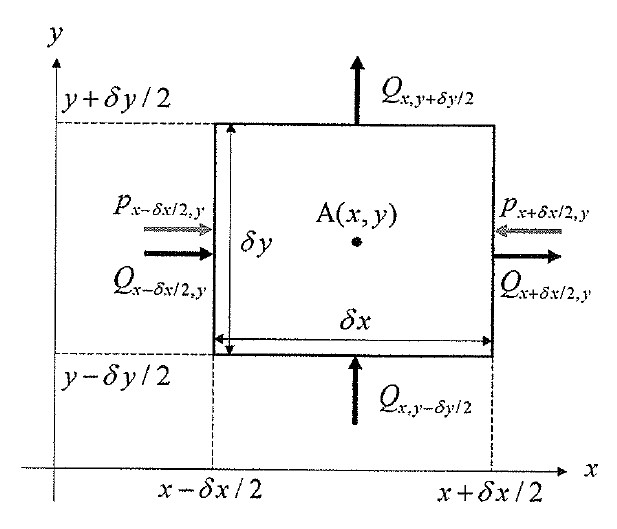
\includegraphics[width=120mm]{images/ryuriki_image1.jpg}
        \caption{R3 試験問題[7]}
    \end{center}
\end{figure}
\subsubsection{2次元の連続の式の導出}
\begin{itembox}[l]{Point}
    \begin{center}
        時刻$t-\delta t/2\leq t \leq t+\delta t/2$の微小時間$\delta t$間の流れについて\textgt{空間}・\textgt{時間}の観点から保存則を立てる
    \end{center}
\end{itembox}
図1において,連続の式を導出する.
\noindent$\delta t$間に流入する流体の質量を$M_{in}$,$\delta t$間に流出する流体の質量を$M_{out}$,$\delta t$間の質量増加量を$\Delta M$とすると,\\
・\textgt{流入・流出量(空間的観点)}
\begin{eqnarray*}
    M_{in}&=&\left(\rho u\right)_{x-\frac{1}{2}\delta x}\delta y \delta t+\left(\rho v\right)_{y-\frac{1}{2}\delta y}\delta x \delta t\\
    M_{out}&=&\left(\rho u\right)_{x+\frac{1}{2}\delta x}\delta y \delta t+\left(\rho v\right)_{y+\frac{1}{2}\delta y}\delta x \delta t\\
\end{eqnarray*}
\noindent
・\textgt{質量増加量(時間的観点)}
\begin{eqnarray*}
    \Delta M=\left(\rho\right)_{t+\frac{1}{2}\delta t}\delta x \delta y-\left(\rho\right)_{t-\frac{1}{2}\delta t}\delta x \delta y
\end{eqnarray*}
質量保存則より,
\begin{eqnarray*}
    (質量増加量)&=&(流入量)-(流出量)\\
    \Delta M&=&\quad M_{in}\quad -\quad M_{out}\\
\end{eqnarray*}
※ 「増加量」は「流入量」$\geq$「流出量」のときに増加する\\
\\
ここで,$\delta x, \delta y, \delta t$のオーダまでTaylor級数展開すると\\
\\
※ ここでは,点$(x,y)$周りの$\left(x,y\right)=\left(x\pm \frac{\delta x}{2},y\pm \frac{\delta y}{2}\right)$のときについて考えている.
\begin{eqnarray*}
    \left(\rho u\right)_{x\pm \frac{1}{2}\delta x}&=&\rho u\pm \frac{\delta x}{2}\frac{\partial\left(\rho u\right)}{\partial x}+O\left(\delta x^2\right)\\
    \left(\rho v\right)_{y\pm \frac{1}{2}\delta y}&=&\rho v\pm \frac{\delta y}{2}\frac{\partial\left(\rho v\right)}{\partial y}+O\left(\delta y^2\right)\\
    \left(\rho\right)_{t\pm \frac{1}{2}\delta t}&=&\rho \pm \frac{\delta t}{2}\frac{\partial \rho}{\partial t}+O\left(\delta t^2\right)
\end{eqnarray*}
したがって,上式を代入すると,
\begin{eqnarray*}
    \dfrac{\partial \rho}{\partial t}\delta x \delta y \delta t&=&-\left(\frac{\partial\left(\rho u\right)}{\partial x}+\frac{\partial\left(\rho v\right)}{\partial y}\right)\delta x \delta y \delta t\\
\end{eqnarray*}
これを変形して,
\begin{eqnarray*}
    \dfrac{\partial p}{\partial t}+\frac{\partial\left(\rho u\right)}{\partial x}+\frac{\partial\left(\rho v\right)}{\partial y}&=&0
\end{eqnarray*}
以上より,2次元空間における連続の式を導くことができた.
\subsubsection{2次元のオイラーの運動方程式の導出}
\begin{itembox}[l]{Point}
    \begin{center}
        \textgt{ニュートンの第二法則}\quad$F=ma$を流体について立てる
    \end{center}
\end{itembox}
\textgt{($x$方向)}\\
・\textgt{流体の質量:$m$}\\
\begin{eqnarray*}
    m=\rho \delta x \delta y
\end{eqnarray*}
・\textgt{加速度:$a$}\\
$x$方向の速度$u$の全微分$du$は,
\begin{eqnarray*}
    du=\dfrac{\partial u}{\partial x}dx+\dfrac{\partial u}{\partial y}dy+\dfrac{\partial u}{\partial t}dt
\end{eqnarray*}
\subsubsection{ハーゲン・ポアズイユ流}
断面積が一定の円管内をゆっくりと流れる流れのことを\textgt{ハーゲン・ポアズイユ流}という。\\
ナビエ・ストークス方程式を解析的に解くことができる数少ない厳密解の1つ。
\begin{itembox}[l]{ハーゲン・ポアズイユ流}
    \begin{eqnarray*}
        u\left(r\right)&=&-\frac{1}{4\mu}\left(\frac{dp}{dx}\right)\left(r_0^2-r^2\right)\\
        r_0\; &:&\; 円管の半径\\
    \end{eqnarray*}
\end{itembox}
\subsection{流体のせん断応力}
流体の流れに平行な軸を$x$軸,垂直な軸を$y$とすると,せん断応力$\tau\left(y\right)$は以下のように表せる.
\begin{itembox}[l]{せん断応力(2次元)}
    \begin{eqnarray*}
        \tau\left(y\right)=\mu\dfrac{du}{dy}\\
    \end{eqnarray*}
\end{itembox}
\subsubsection{(例題) 板が流体から受ける力}
\begin{itembox}[l]{Point}
    \begin{center}
        \textgt{下の物体}が、\textgt{上の物体}から受ける力
    \end{center}
\end{itembox}
\subsection{応力テンソル}
\begin{itembox}[l]{二次元非圧縮流体における応力テンソル}
    \begin{eqnarray*}
        \sigma_{ij}=-\delta_{ij}P+\mu\left(\frac{\partial u_i}{\partial x_j}+\frac{\partial u_j}{\partial x_i}\right)\\
    \end{eqnarray*}
\end{itembox}
\begin{itembox}[l]{それぞれの応力成分}
    \begin{eqnarray*}
        \sigma_{xx} &=& -P+2\mu\left(\frac{\partial u}{\partial x}\right)\\
        \sigma_{yy} &=& -P+2\left(\frac{\partial v}{\partial y}\right)\\
        \sigma_{xy} &=& \mu\left(\frac{\partial u}{\partial y}+\frac{\partial v}{\partial x}\right)\\
        \sigma_{yx} &=& \mu\left(\frac{\partial v}{\partial x}+\frac{\partial u}{\partial y}\right)\\
    \end{eqnarray*}
\end{itembox}
\subsection{レイノルズ数}
\begin{itembox}[l]{レイノルズ数}
    \begin{eqnarray*}
        \mathrm{Re}&=&\dfrac{UL}{\nu}\\
        \mathrm{Re} &:& レイノルズ数\\
        U &:& 代表速度\\
        L &:& 代表長さ\\
        \nu &:& 動粘性係数\\
    \end{eqnarray*}
\end{itembox}
\subsection{流れ場の幾何学的表現}
流れ場を表現する手法として\textgt{流線}・\textgt{流跡線}・\textgt{流脈線}という概念がある.\\
\subsubsection{流線}
流線は,時間$t$をある時刻に固定し,その時刻における速度ベクトルが接線ベクトルとなる曲線のことである.\\
つまり,$\vec{u}\parallel d\vec{x}$が成立する.
\begin{itembox}[l]{流線}
    \begin{eqnarray*}
        \dfrac{dx}{u}&=&\dfrac{dy}{v}=\dfrac{dz}{w}\\
        vdx&-&udy=0\quad (2次元)\\
    \end{eqnarray*}
\end{itembox}
流線が交差するとき,その交点では流体は速度ゼロもしくは無限大をとる.
速度がゼロのとき,その交点を\textgt{よどみ点}といい,無限大のとき\textgt{特異点}という.
また,この流線によって作られる曲面を\textgt{流管}という.
\subsubsection{流跡線}
流跡線は,流体粒子を時間とともにラグランジュ的に追跡したときに描かれる軌跡を示す概念であり,以下のように表される.
\begin{itembox}[l]{流跡線}
    \begin{eqnarray*}
        d\vec{x}=\vec{u}dt\\
    \end{eqnarray*}
\end{itembox}
\subsubsection{流脈}
空間のある点を通過した流体のすべての粒子が任意の瞬間に存在する点を結んだ線のこと.\\
例) たばこの煙をある瞬間に撮影したもの
\subsection{渦度}
流れ場の回転の程度を表す量を\textgt{渦度}という.
$\vec{u}=\left(u,v\right)$のとき,以下のように表される.
\begin{itembox}[l]{渦度}
    \begin{eqnarray*}
        \zeta = rot\;\vec{u}=\dfrac{\partial v}{\partial x}-\dfrac{\partial u}{\partial y}\\
    \end{eqnarray*}
\end{itembox}
また,渦度$\zeta$は回転の角速度$\omega$の2倍に等しい.
\begin{eqnarray*}
    \omega = \dfrac{1}{2}\zeta
\end{eqnarray*}
ここで,$\zeta=0$のとき,回転のない運動(\textgt{渦なし流れ})となる.これを\textgt{ポテンシャル流}という.
\subsection{流れ関数}
以下の条件を満たす関数$\psi$を\textgt{流れ関数}という.
\begin{itembox}[l]{流れ関数}
    \begin{eqnarray*}
        u=\dfrac{\partial \psi}{\partial y}\quad v=-\dfrac{\partial \psi}{\partial x}\\
    \end{eqnarray*}
\end{itembox}
$\psi =const$のとき,全微分をとると\\
\begin{eqnarray*}
    d\psi = \dfrac{\partial \psi}{\partial x}dx+\dfrac{\partial \psi}{\partial y}dy=0\\
\end{eqnarray*}
これは,流線の定義と同じになっていることがわかる.すなわち,$\psi = const$は流線を表す.\\
※ 流線と関係が深い → 流れの方向ベクトルを表すことができる.
\subsection{速度ポテンシャル}
以下の条件を満たす関数$\phi$を\textgt{速度ポテンシャル}という.
また,このとき流れは\textgt{渦なし流れ}である必要がある.
\begin{itembox}[l]{速度ポテンシャル}
    \begin{eqnarray*}
        u=\dfrac{\partial \phi}{\partial x}\quad v=\dfrac{\partial \phi}{\partial y}\\
    \end{eqnarray*}
\end{itembox}
速度ポテンシャル$\phi = const$の曲線を\textgt{等ポテンシャル線}と呼ぶ.\\
※ 渦度$\zeta$と関係が深い → 流れに渦(回転運動)がない状態のことを表すことができる
\subsection{コーシー・リーマンの関係式}
\textgt{定常かつ渦なし流れ}のとき,以下の関係(\textgt{コーシー・リーマンの関係式})が成立する.
\begin{itembox}[l]{コーシー・リーマンの関係式}
    \begin{eqnarray*}
        u&=&\dfrac{\partial \phi}{\partial x}=\dfrac{\partial \psi}{\partial y}\\
        v&=&\dfrac{\partial \phi}{\partial y}=-\dfrac{\partial \psi}{\partial x}\\
    \end{eqnarray*}
\end{itembox}
これは,$\phi$と$\psi$の直交性を示す.
すなわち,流線($\psi=zconst$)と等ポテンシャル線($\phi=const$)は直交する.
\subsubsection{直交性の証明}
コーシー・リーマンの関係式が成立するとき,
$\psi=const\quad \phi=const$の法線ベクトルはそれぞれ,
\begin{eqnarray*}
    grad \psi&=&\left(\dfrac{\partial \psi}{\partial x}, \dfrac{\partial \psi}{\partial y}\right)\\
    grad \phi&=&\left(\dfrac{\partial \phi}{\partial x}, \dfrac{\partial \phi}{\partial y}\right)
\end{eqnarray*}
これらの内積を計算すると,
\begin{eqnarray*}
    grad\psi \cdot grad\phi &=& \dfrac{\partial \psi}{\partial x}\dfrac{\partial \phi}{\partial x} +\dfrac{\partial \psi}{\partial y}\dfrac{\partial \phi}{\partial y}\\
    &=&\dfrac{\partial \phi}{\partial x}\left(-\dfrac{\partial \phi}{\partial y}\right)+\dfrac{\partial \phi}{\partial y}\dfrac{\partial \phi}{\partial x}\\
    &=&0
\end{eqnarray*}
したがって,2つの法線ベクトルは直行しているといえる.よって,流れ関数$\psi$と速度ポテンシャル$\phi$の直交性は示された.
\end{document}